%%%%%%%%%%%%%%%%%%%%%%%%%%%%%%%%%%%%%%%%%
% The Legrand Orange Book
% LaTeX Template
% Version 1.2 (19/5/13)
%
% This template has been downloaded from:
% http://www.LaTeXTemplates.com
%
% Original author:
% Mathias Legrand (legrand.mathias@gmail.com)
%
% License:
% CC BY-NC-SA 3.0 (http://creativecommons.org/licenses/by-nc-sa/3.0/)
%
% Compiling this template:
% This template uses biber for its bibliography and makeindex for its index.
% This means that to update the bibliography and index in this template you
% will need to run the following sequence of commands in the template
% directory:
%
% 1) pdflatex skillmanual
% 2) makeindex skillmanual.idx -s StyleInd.ist
% 3) biber skillmanual
% 4) pdflatex skillmanual
%
% This template also uses a number of packages which may need to be
% updated to the newest versions for the template to compile. It is strongly
% recommended you update your LaTeX distribution if you have any
% compilation errors.
%
% Important note:
% Chapter heading images should have a 2:1 width:height ratio,
% e.g. 920px width and 460px height.
%
%%%%%%%%%%%%%%%%%%%%%%%%%%%%%%%%%%%%%%%%%

%----------------------------------------------------------------------------------------
%	PACKAGES AND OTHER DOCUMENT CONFIGURATIONS
%----------------------------------------------------------------------------------------

\documentclass[11pt]{book} % Default font size and left-justified equations

\usepackage[top=3cm,bottom=3cm,left=2.5cm,right=2.5cm,headsep=10pt,a4paper]{geometry} % Page margins

\usepackage{xcolor} % Required for specifying colors by name
\definecolor{ocre}{RGB}{207,83,0} % Define the orange color used for highlighting throughout the book

\usepackage{listings}
\lstloadlanguages{[5.2]Mathematica}
% Font Settings
\usepackage{avant} % Use the Avantgarde font for headings
%\usepackage{times} % Use the Times font for headings
\usepackage{mathptmx} % Use the Adobe Times Roman as the default text font together with math symbols from the Sym­bol, Chancery and Com­puter Modern fonts
%\usepackage{courier}
\usepackage{framed}
\usepackage{float}
\usepackage{microtype} % Slightly tweak font spacing for aesthetics
\usepackage[utf8]{inputenc} % Required for including letters with accents
\usepackage[T1]{fontenc} % Use 8-bit encoding that has 256 glyphs
\usepackage{amsmath}
\usepackage{csquotes}
\usepackage[ampersand]{easylist}
\usepackage{tabularx}
\usepackage{url}
% Bibliography
\usepackage[style=alphabetic,sorting=nyt,sortcites=true,autopunct=true,babel=hyphen,hyperref=true,abbreviate=false,backref=true,backend=biber]{biblatex}
\addbibresource{bibliography.bib} % BibTeX bibliography file
\defbibheading{bibempty}{}

% Index
\usepackage{calc} % For simpler calculation - used for spacing the index letter headings correctly
\usepackage{makeidx} % Required to make an index
\makeindex % Tells LaTeX to create the files required for indexing


% Quotes

\newenvironment{aquote}[1]{%
  \pushQED{#1}%
  \begin{quote}
}{%
  \par\nointerlineskip\noindent\hfill\popQED%
  \end{quote}%
}

\newcommand*{\avantfont}{\fontfamily{pag}\selectfont}
%----------------------------------------------------------------------------------------

%----------------------------------------------------------------------------------------
%	VARIOUS REQUIRED PACKAGES
%----------------------------------------------------------------------------------------

\usepackage{titlesec} % Allows customization of titles

\usepackage{graphicx} % Required for including pictures
\graphicspath{{./Pictures/}} % Specifies the directory where pictures are stored

\usepackage{lipsum} % Inserts dummy text

\usepackage{tikz} % Required for drawing custom shapes

\usepackage[english]{babel} % English language/hyphenation

\usepackage{enumitem} % Customize lists
\setlist{nolistsep} % Reduce spacing between bullet points and numbered lists

\usepackage{booktabs} % Required for nicer horizontal rules in tables

\usepackage{eso-pic} % Required for specifying an image background in the title page

%----------------------------------------------------------------------------------------
%	MAIN TABLE OF CONTENTS
%----------------------------------------------------------------------------------------

\usepackage{titletoc} % Required for manipulating the table of contents

\contentsmargin{0cm} % Removes the default margin
% Chapter text styling
\titlecontents{chapter}[1.25cm] % Indentation
{\addvspace{15pt}\large\sffamily\bfseries} % Spacing and font options for chapters
{\color{ocre!60}\contentslabel[\Large\thecontentslabel]{1.25cm}\color{ocre}} % Chapter number
{}  
{\color{ocre!60}\normalsize\sffamily\bfseries\;\titlerule*[.5pc]{.}\;\thecontentspage} % Page number
% Section text styling
\titlecontents{section}[1.25cm] % Indentation
{\addvspace{5pt}\sffamily\bfseries} % Spacing and font options for sections
{\contentslabel[\thecontentslabel]{1.25cm}} % Section number
{}
{\sffamily\hfill\color{black}\thecontentspage} % Page number
[]
% Subsection text styling
\titlecontents{subsection}[1.25cm] % Indentation
{\addvspace{1pt}\sffamily\small} % Spacing and font options for subsections
{\contentslabel[\thecontentslabel]{1.25cm}} % Subsection number
{}
{\sffamily\;\titlerule*[.5pc]{.}\;\thecontentspage} % Page number
[] 

%----------------------------------------------------------------------------------------
%	MINI TABLE OF CONTENTS IN CHAPTER HEADS
%----------------------------------------------------------------------------------------

% Section text styling
\titlecontents{lsection}[0em] % Indendating
{\footnotesize\sffamily} % Font settings
{}
{}
{}

% Subsection text styling
\titlecontents{lsubsection}[.5em] % Indentation
{\normalfont\footnotesize\sffamily} % Font settings
{}
{}
{}
 
%----------------------------------------------------------------------------------------
%	PAGE HEADERS
%----------------------------------------------------------------------------------------

\usepackage{fancyhdr} % Required for header and footer configuration

\pagestyle{fancy}
\renewcommand{\chaptermark}[1]{\markboth{\sffamily\normalsize\bfseries #1}{}} % Chapter text font settings
\renewcommand{\sectionmark}[1]{\markright{\sffamily\normalsize\thesection\hspace{5pt}#1}{}} % Section text font settings
\fancyhf{} \fancyhead[LE,RO]{\sffamily\normalsize\thepage} % Font setting for the page number in the header
\fancyhead[LO]{\rightmark} % Print the nearest section name on the left side of odd pages
\fancyhead[RE]{\leftmark} % Print the current chapter name on the right side of even pages
\renewcommand{\headrulewidth}{0.5pt} % Width of the rule under the header
\addtolength{\headheight}{2.5pt} % Increase the spacing around the header slightly
\renewcommand{\footrulewidth}{0pt} % Removes the rule in the footer
\fancypagestyle{plain}{\fancyhead{}\renewcommand{\headrulewidth}{0pt}} % Style for when a plain pagestyle is specified

% Removes the header from odd empty pages at the end of chapters
\makeatletter
\renewcommand{\cleardoublepage}{
\clearpage\ifodd\c@page\else
\hbox{}
\vspace*{\fill}
\thispagestyle{empty}
\newpage
\fi}

%----------------------------------------------------------------------------------------
%	THEOREM STYLES
%----------------------------------------------------------------------------------------

\usepackage{amsmath,amsfonts,amssymb,amsthm} % For including math equations, theorems, symbols, etc

\newcommand{\intoo}[2]{\mathopen{]}#1\,;#2\mathclose{[}}
\newcommand{\ud}{\mathop{\mathrm{{}d}}\mathopen{}}
\newcommand{\intff}[2]{\mathopen{[}#1\,;#2\mathclose{]}}
\newtheorem{notation}{Notation}[chapter]

\newtheoremstyle{ocrenum} % Theorem style name
{7pt} % Space above
{7pt} % Space below
{\normalfont} % Body font
{} % Indent amount
{\small\bf\sffamily\color{ocre}} % Theorem head font
{\;\; \\} % Punctuation after theorem head
{0.25em} % Space after theorem head
{\small\sffamily\color{ocre}\thmname{#1}\thmnumber{\@ifnotempty{#1}{ }\@upn{#2}} % Theorem text (e.g. Theorem 2.1)
\thmnote{\ {\the\thm@notefont\sffamily\bfseries\color{black}--- #3.}}} % Optional theorem note
\renewcommand{\qedsymbol}{$\blacksquare$} % Optional qed square

\newtheoremstyle{blacknumex} % Theorem style name
{7pt} % Space above
{7pt} % Space below
{\normalfont} % Body font
{} % Indent amount
{\small\bf\sffamily} % Theorem head font
{\;\; } % Punctuation after theorem head
{0.25em} % Space after theorem head
{\small\sffamily{\tiny\ensuremath{\blacksquare}}\ \thmname{#1}\thmnumber{\@ifnotempty{#1}{ }\@upn{#2}} % Theorem text (e.g. Theorem 2.1)
\thmnote{\ {\the\thm@notefont\sffamily\bfseries--- #3.}}} % Optional theorem note

\newtheoremstyle{blacknum} % Theorem style name
{7pt} % Space above
{7pt} % Space below
{\normalfont} % Body font
{} % Indent amount
{\small\bf\sffamily} % Theorem head font
{\;\;} % Punctuation after theorem head
{0.25em} % Space after theorem head
{\small\sffamily\thmname{#1}\thmnumber{\@ifnotempty{#1}{ }\@upn{#2}} % Theorem text (e.g. Theorem 2.1)
\thmnote{\ {\the\thm@notefont\sffamily\bfseries--- #3.}}} % Optional theorem note
\makeatother

% Defines the theorem text style for each type of theorem to one of the three styles above
\theoremstyle{ocrenum}
\newtheorem{theoremeT}{Theorem}[chapter]
\newtheorem{proposition}{Proposition}[chapter]
\newtheorem{problem}{Problem}[chapter]
\newtheorem{exerciseT}{Useful Tip}[chapter]
\theoremstyle{blacknumex}
\newtheorem{exampleT}{Example}[chapter]
\theoremstyle{blacknum}
\newtheorem{vocabulary}{Vocabulary}[chapter]
\newtheorem{definitionT}{Definition}[chapter]
\newtheorem{corollaryT}{Code Example}[chapter]

%----------------------------------------------------------------------------------------
%	DEFINITION OF COLORED BOXES
%----------------------------------------------------------------------------------------

\RequirePackage[framemethod=default]{mdframed} % Required for creating the theorem, definition, exercise and corollary boxes

% Theorem box
\newmdenv[skipabove=7pt,
skipbelow=7pt,
backgroundcolor=black!5,
linecolor=ocre,
innerleftmargin=5pt,
innerrightmargin=5pt,
innertopmargin=5pt,
leftmargin=0cm,
rightmargin=0cm,
innerbottommargin=5pt]{tBox}

% Exercise box	  
\newmdenv[skipabove=7pt,
skipbelow=7pt,
rightline=false,
leftline=true,
topline=false,
bottomline=false,
backgroundcolor=ocre!10,
linecolor=ocre,
innerleftmargin=5pt,
innerrightmargin=5pt,
innertopmargin=5pt,
innerbottommargin=5pt,
leftmargin=0cm,
rightmargin=0cm,
linewidth=4pt]{eBox}	

% Definition box
\newmdenv[skipabove=10pt,
skipbelow=10pt,
rightline=false,
leftline=true,
topline=false,
bottomline=false,
linecolor=ocre,
innerleftmargin=5pt,
innerrightmargin=5pt,
innertopmargin=0pt,
leftmargin=0cm,
rightmargin=0cm,
linewidth=4pt,
innerbottommargin=0pt]{dBox}	

% Corollary box
\newmdenv[skipabove=7pt,
skipbelow=7pt,
rightline=false,
leftline=true,
topline=false,
bottomline=false,
linecolor=gray,
backgroundcolor=black!5,
innerleftmargin=5pt,
innerrightmargin=5pt,
innertopmargin=5pt,
leftmargin=0cm,
rightmargin=0cm,
linewidth=4pt,
innerbottommargin=5pt]{cBox}				  
		  

% Creates an environment for each type of theorem and assigns it a theorem text style from the "Theorem Styles" section above and a colored box from above
\newenvironment{theorem}{\begin{tBox}\begin{theoremeT}}{\end{theoremeT}\end{tBox}}
\newenvironment{exercise}{\begin{eBox} \begin{exerciseT}}{\end{exerciseT}\end{eBox}}				  
\newenvironment{definition}{\begin{dBox}\begin{definitionT}}{\end{definitionT}\end{dBox}}	
\newenvironment{example}{\begin{exampleT}}{\end{exampleT}}		
\newenvironment{corollary}{\begin{cBox}\begin{corollaryT}}{\end{corollaryT}\end{cBox}}	

%----------------------------------------------------------------------------------------
%	REMARK ENVIRONMENT
%----------------------------------------------------------------------------------------

\newenvironment{remark}{\par\vskip10pt\small % Vertical white space above the remark and smaller font size
\begin{list}{}{
\leftmargin=35pt % Indentation on the left
\rightmargin=25pt}\item\ignorespaces % Indentation on the right
\makebox[-2.5pt]{\begin{tikzpicture}[overlay]
\node[draw=ocre!60,line width=1pt,circle,fill=ocre!25,font=\sffamily\bfseries,inner sep=2pt,outer sep=0pt] at (-15pt,0pt){\textcolor{ocre}{R}};\end{tikzpicture}} % Orange R in a circle
\advance\baselineskip -1pt}{\end{list}\vskip5pt} % Tighter line spacing and white space after remark

%--------------------------------------------------------------------------------------
%	SECTION NUMBERING IN THE MARGIN
%----------------------------------------------------------------------------------------

\makeatletter
\renewcommand{\@seccntformat}[1]{\llap{\textcolor{ocre}{\csname the#1\endcsname}\hspace{1em}}}                    
\renewcommand{\section}{\@startsection{section}{1}{\z@}
{-4ex \@plus -1ex \@minus -.4ex}
{1ex \@plus.2ex }
{\normalfont\large\sffamily\bfseries}}
\renewcommand{\subsection}{\@startsection {subsection}{2}{\z@}
{-3ex \@plus -0.1ex \@minus -.4ex}
{0.5ex \@plus.2ex }
{\normalfont\sffamily\bfseries}}
\renewcommand{\subsubsection}{\@startsection {subsubsection}{3}{\z@}
{-2ex \@plus -0.1ex \@minus -.2ex}
{0.2ex \@plus.2ex }
{\normalfont\small\sffamily\bfseries}}                        
\renewcommand\paragraph{\@startsection{paragraph}{4}{\z@}
{-2ex \@plus-.2ex \@minus .2ex}
{0.1ex}
{\normalfont\small\sffamily\bfseries}}

%----------------------------------------------------------------------------------------
%	CHAPTER HEADINGS
%----------------------------------------------------------------------------------------

\newcommand{\thechapterimage}{}
\newcommand{\chapterimage}[1]{\renewcommand{\thechapterimage}{#1}}
\def\thechapter{\arabic{chapter}}
\def\@makechapterhead#1{
\thispagestyle{empty}
{\centering \normalfont\sffamily
\ifnum \c@secnumdepth >\m@ne
\if@mainmatter
\startcontents
\begin{tikzpicture}[remember picture,overlay]
\node at (current page.north west)
{\begin{tikzpicture}[remember picture,overlay]

\node[anchor=north west,inner sep=0pt] at (0,0) {\includegraphics[width=\paperwidth]{\thechapterimage}};

%Commenting the 3 lines below removes the small contents box in the chapter heading
\draw[fill=white,opacity=.6] (1cm,0) rectangle (8cm,-7cm);
\node[anchor=north west] at (1cm,.25cm) {\parbox[t][8cm][t]{6.5cm}{\huge\bfseries\flushleft \printcontents{l}{1}{\setcounter{tocdepth}{2}}}};

\draw[anchor=west] (5cm,-9cm) node [rounded corners=25pt,fill=white,fill opacity=.6,text opacity=1,draw=ocre,draw opacity=1,line width=2pt,inner sep=15pt]{\huge\sffamily\bfseries\textcolor{black}{\thechapter\ ---\ #1\vphantom{plPQq}\makebox[22cm]{}}};
\end{tikzpicture}};
\end{tikzpicture}}\par\vspace*{230\p@}
\fi
\fi
}
\def\@makeschapterhead#1{
\thispagestyle{empty}
{\centering \normalfont\sffamily
\ifnum \c@secnumdepth >\m@ne
\if@mainmatter
\startcontents
\begin{tikzpicture}[remember picture,overlay]
\node at (current page.north west)
{\begin{tikzpicture}[remember picture,overlay]
\node[anchor=north west] at (-4pt,4pt) {\includegraphics[width=\paperwidth]{\thechapterimage}};
\draw[anchor=west] (5cm,-9cm) node [rounded corners=25pt,fill=white,opacity=.7,inner sep=15.5pt]{\huge\sffamily\bfseries\textcolor{black}{\vphantom{plPQq}\makebox[22cm]{}}};
\draw[anchor=west] (5cm,-9cm) node [rounded corners=25pt,draw=ocre,line width=2pt,inner sep=15pt]{\huge\sffamily\bfseries\textcolor{black}{#1\vphantom{plPQq}\makebox[22cm]{}}};
\end{tikzpicture}};
\end{tikzpicture}}\par\vspace*{230\p@}
\fi
\fi
}
\makeatother % Insert the commands.tex file which contains the majority of the structure behind the template

\usepackage{hyperref}
\hypersetup{hidelinks,backref=true,pagebackref=true,hyperindex=true,colorlinks=false,breaklinks=true,urlcolor= blue,bookmarks=true,bookmarksopen=false,pdftitle={book title},pdfauthor={book author}}
% compression pdf
\pdfminorversion=5
\pdfobjcompresslevel=6 
\pdfcompresslevel=9


\begin{document}

%----------------------------------------------------------------------------------------
%	TITLE PAGE
%----------------------------------------------------------------------------------------

\begingroup
\thispagestyle{empty}
\AddToShipoutPicture*{\put(6,5){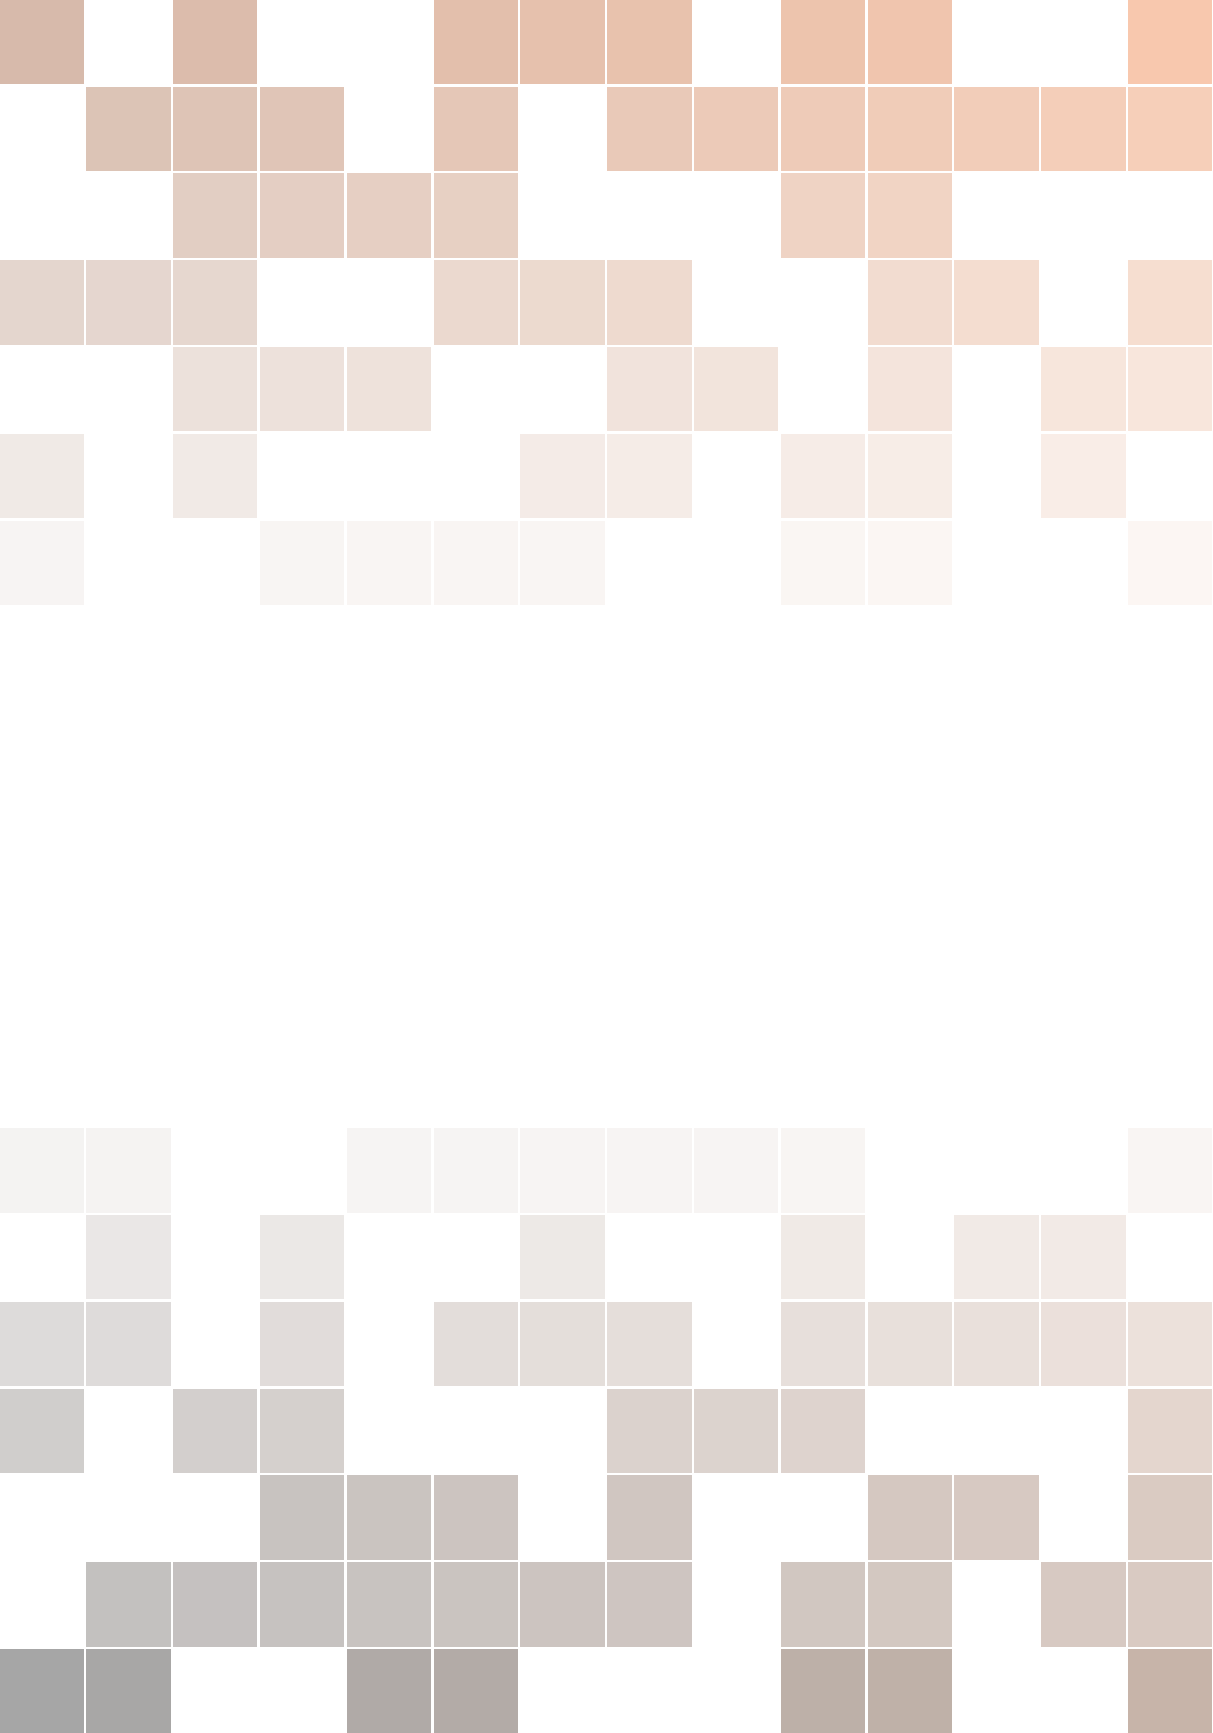
\includegraphics[scale=1]{background}}} % Image background
\centering
\vspace*{9cm}
\par\normalfont\fontsize{35}{35}\sffamily\selectfont
Physics Skill Manual \par % Book title
\vspace*{1cm}
{\Huge R. Dawson Baker}\par % Author name
\endgroup

%----------------------------------------------------------------------------------------
%	COPYRIGHT PAGE
%----------------------------------------------------------------------------------------

\newpage
~\vfill
\thispagestyle{empty}

\noindent Copyright \copyright\ 2013 R. Dawson Baker\\ % Copyright notice

\noindent \textsc{Published by Publisher}\\ % Publisher

\noindent \textsc{book-website.com}\\ % URL

\noindent Licensed under the Creative Commons Attribution-NonCommercial 3.0 Unported License (the ``License''). You may not use this file except in compliance with the License. You may obtain a copy of the License at \url{http://creativecommons.org/licenses/by-nc/3.0}. Unless required by applicable law or agreed to in writing, software distributed under the License is distributed on an \textsc{``AS IS'' BASIS, WITHOUT WARRANTIES OR CONDITIONS OF ANY KIND}, either express or implied. See the License for the specific language governing permissions and limitations under the License.\\ % License information

\noindent \textit{First printing, March 2013} % Printing/edition date

%----------------------------------------------------------------------------------------
%	TABLE OF CONTENTS
%----------------------------------------------------------------------------------------

\chapterimage{chapter_head_1.pdf} % Table of contents heading image

\pagestyle{empty} % No headers

\tableofcontents % Print the table of contents itself

\cleardoublepage % Forces the first chapter to start on an odd page so it's on the right

\pagestyle{fancy} % Print headers again

%----------------------------------------------------------------------------------------
%	Introduction
%----------------------------------------------------------------------------------------

\chapterimage{chapter_head_1.pdf} % Chapter heading image

\chapter{Introduction}


This document was originally created by R. Dawson Baker as a basis for the skills students need to excel in the ``Modern Lab'' or ``Junior Lab'' PHY 353L course at the University
of Texas at Austin. It is currently maintained by the local chapters of the Society of Physics Students and Sigma Pi Sigma, the physics honors society.

\section{Contact Information}

Find an error in this document? Or something that needs to be updated? Instructions unclear? Code not compiling? Let us know! You can email the officers of SPS at spsofficers@gmail.com
or express your concerns to your TA and they will pass them along.

\section{Resources}

The Society of Physics Students maintains some additional resources that may be found at \url{http://www.ph.utexas.edu/~sps}.

In particular, a handy template for use in the Modern Lab (originally created by UT Physics student Johnathan Blair) can be found at \url{http://www.ph.utexas.edu/~sps/resources/Modern_Lab_LaTeX_Template.tex}
%----------------------------------------------------------------------------------------
%	Typesetting papers and documents in LaTeX
%----------------------------------------------------------------------------------------

\chapterimage{chapter_head_1.pdf} % Chapter heading image

\chapter{Typesetting documents in \LaTeX}


\LaTeX (pronounced ``lah-tech'' or `` lay-tech'') is a mark-up language that allows an author to specifically, precisely and easily specify how layout and content are combined. It is based on Dr. Donald Knuth's \TeX typesetting system with two goals in mind:\\


\begin{enumerate}
\item It should  be easy a require only a ``minimal amount of effort'' for the author to produce high-quality documents, and
\item It should run on every operating system.\\
\end{enumerate}

Both these goals have been essentially accomplished, resulting in wide-spread use among the scientific community. At this point -- while there are alternatives for typesetting scientific documents  --  \LaTeX\ can easily be considered a basic tool that every physicist should get to know well. Besides making equations look good, the mark-up language is commonly used for:\\


\begin{enumerate}
\item {\bf Making digital and hard-copy media}. This book itself was typeset in \LaTeX.
\item {\bf Making navigable documents by using hyperlinks in a pdf}. This means that you can click on certain words in the document and it will take you to another place in the document, another document, or even a website.
\item {\bf Making high quality documents whose fonts and images can be scaled to be printed on many different kinds of printers}.\\
\end{enumerate}
These features, combined with the fact that the language is open-source and free to use, have made \LaTeX\ a staple in the world of publishing and scientific journals. For instance, many scientific journals prefer or exclusively accept documents in \LaTeX\ code because it is so easy to get to a finished product, and \LaTeX\ documents contain all the information necessary to render the product regardless of platform. If you are considering submitting something to the ArXiv (a well known open-access database for preprints) at some point, you \emph{should} know \LaTeX\ . While you \emph{could} get by without it, very few people do.

%\begin{framed}
{\bf To help you get to know \LaTeX , this book will focus on three things: (1) explaining the basics in what is hoped is a concise way, (2) pointing you towards good online resources on the subject if you're confused and (3) (if you're up to it) helping you to get started with REV\TeX , a package tailored specifically to the needs of physicists.}
%\end{framed}

\section{Getting \LaTeX\ -- compilers and editors}

To use \LaTeX, you need to (1) download the compiler for your operating system, then (2) download a \LaTeX\ editor that you like. The compiler is the program which does the actual typesetting by creating a \texttt{.pdf} file, and it is different for every operating system:\\
\begin{enumerate}
\item Microsoft Windows $\implies$ MikTeX: \url{http://miktex.org/}
\item Mac OS $\implies$ MacTeX: \url{http://tug.org/mactex/}
\item Linux $\implies$ look for the \texttt{texlive} package in your package manager.\\
\end{enumerate}
There are \emph{many} \LaTeX\ editors, each of them has its own advantages and disadvantages. Some of the favorites at UT are \footnote{This book was typeset using Texmaker. The hotkeys and structure manager came in very handy when working through a lot of code and trying to manage multiple chapters.}:
\begin{figure}[h]
\centering
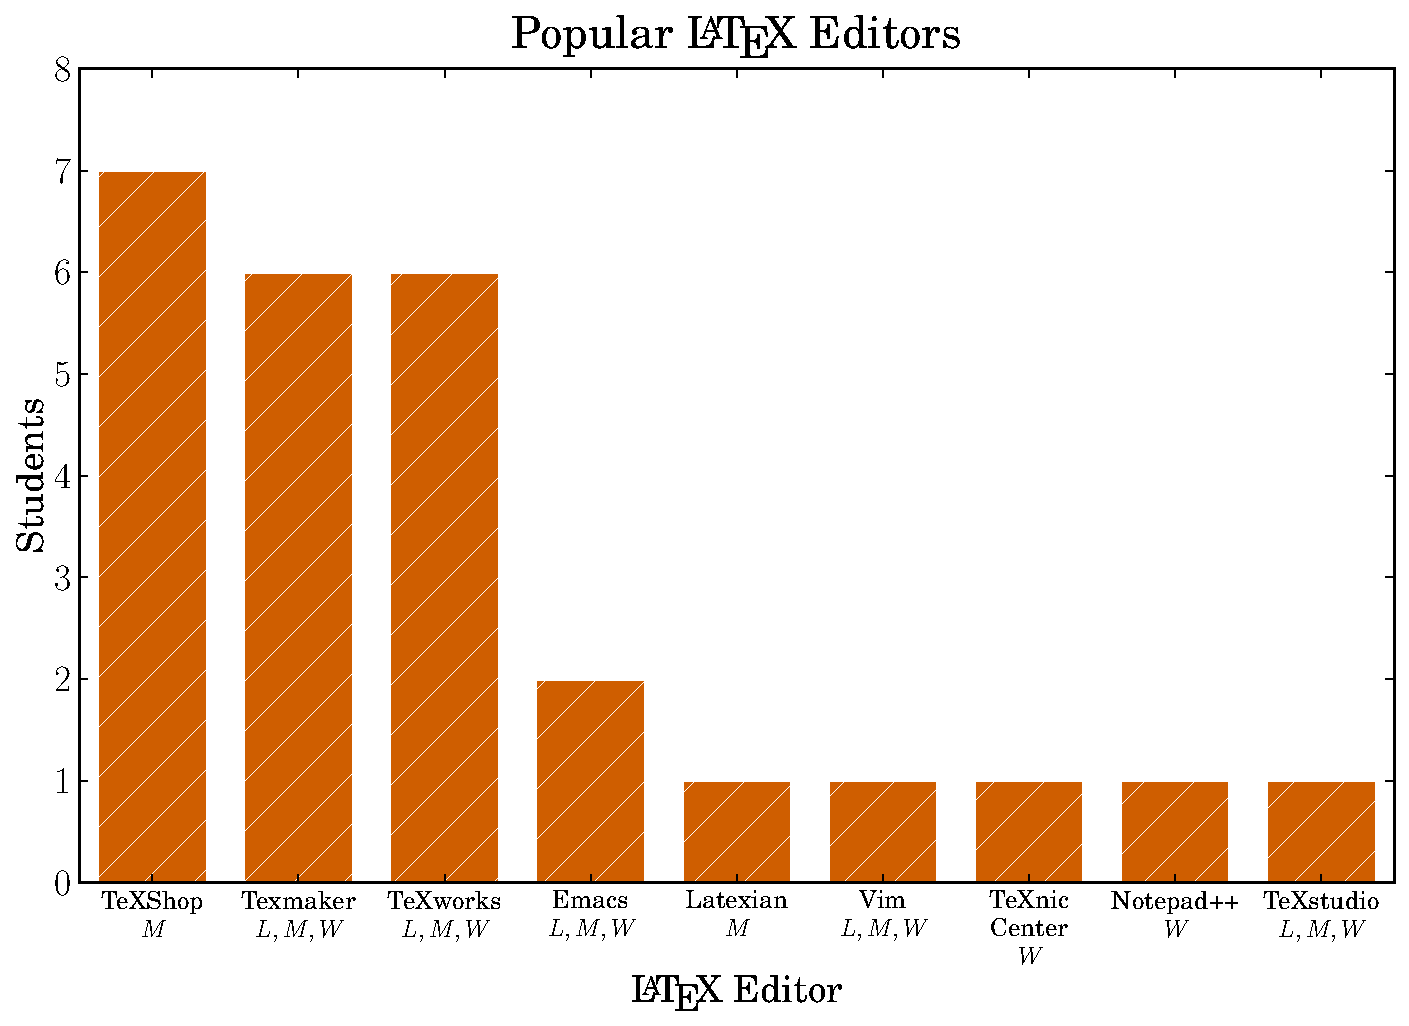
\includegraphics[scale=.675]{editorprefs.pdf}
\caption{A Facebook survey was taken of other UT SPS students' \LaTeX\ editor preferences. The plot above documents the results. Under each editor name, the italicized capital letters show which operating systems the programs are compatible with:  $L$ for Linux, $M$ for Mac OS X, and $W$ for Windows. If you choose one of these, you are most likely to find someone else who knows about the editor you're using (in case you get lost). \emph{Note:} Emacs, Vim, and Notepad++ are text editors that can be modified to run \LaTeX\ code. If you're a serious programmer you may already know what these are. If you're new to \LaTeX\ , it might be best to try something else first.}
\end{figure}

A good compare and contrast of some of the different \LaTeX\ editors out there can be found at \url{http://en.wikipedia.org/wiki/Comparison_of_TeX_editors}

\section{Getting started immediately }
This section is intended to be short and the absolute minimum to get you started with writing a paper in \LaTeX . If you are more interested in a comprehensive introduction you should \emph{certainly} check out these two much more complete guides:

\begin{description}
\item[The \LaTeX\ Wikibook] Found at \url{http://en.wikibooks.org/wiki/LaTeX}, this is probably the best organized and easiest to navigate website. It is slightly more encyclopedic and useful for troubleshooting.
\item[The Not So Short Introduction to \LaTeX 2e] If you're interested in having a \texttt{.pdf} or book reference, \url{http://tobi.oetiker.ch/lshort/lshort.pdf} is a great document that has a lot in common with The \LaTeX\ Wikibook, but is typeset entirely in \LaTeX\ and has a bit more of an attitude.
\end{description}

Both of these references are very similar, and are very enlightening. For a more full understanding of \LaTeX\ (it would be senseless to try to compete with them) you should definitely spend a few hours reading through them. To get writing immediately refer to the document and explanation below.

\subsection{A basic document}
An example of a simple yet functional basic document that has title, abstract, some organization and an equation:


\begin{framed}
\begin{verbatim}
% This is a comment because nothing after a % sign can be displayed. 
\documentclass{article}
\title{This is a title}
\author{Name}
\date{\today}

\begin{document}
\maketitle
\begin{abstract}
This is my abstract
\end{abstract} 
\begin{section}{This is a section}
\begin{subsection}{This is a subsection}
Here is text and below is an equation:
\begin{equation}
\hat H = - \frac{\nabla^2}{2} - \frac{1}{x}
\end{equation}
\end{subsection}
\end{section}
\end{document}
\end{verbatim}
\end{framed}

This code needs to be run for the compiler to yield a document. When run in a \LaTeX\ editor the code produces output that looks like this:

\begin{figure}[H]
\centering
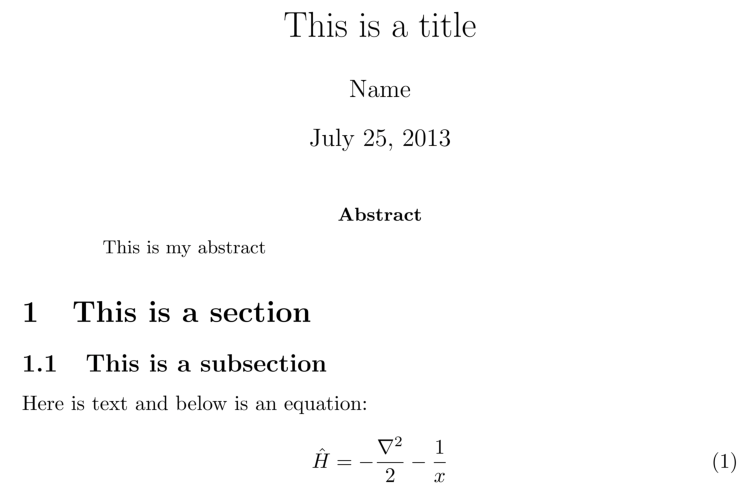
\includegraphics[scale=1]{ex1_crop2.pdf}
\end{figure}
\subsection{Commands and environments}
To understand how this file made it to output, let's look at the general features of the file. First of all, notice that  every word that has a \textbackslash\ in front of it is not displayed. This is because commands in \LaTeX\ start with a backslash. Commands represent blocks of code in \TeX\ , the underlying language that is run to create and render all of the typeset objects that you see in the output document.
Second, notice that every time there is a command of the form \verb|\begin{|  {\it environment} \verb|}|, there is another of the form \verb|\end{| {\it environment} \verb|}| some time later. This is because these commands delimit ( set the bounds of ) blocks of code called ``environments". Environments are spaces in which all code is interpreted in a specific way. Some commands and environments therefore only make sense or can be used within certain kinds of environments. By thinking in terms of {\it commands} and {\it environments}, \LaTeX\ translates a few words into a lot of specific \TeX\ commands that we would really rather not see (because they are incredibly tedious). This is why the system is so powerful: you only need to give \LaTeX\ your content, and it does all the formatting according to rules you can understand and tinker with. {\bf Learning how to use the system well is therefore really just a matter of understanding how the existing rules work and how new rules are made.}



\section{How the existing rules work}

The undisputed best way to understand how the rules of \LaTeX\ work is to actually try to write some files. While this is true, it is handy to know about the basic structure and conventions of a \texttt{.tex} document when searching for documentation and for imitating examples found online. This section will therefore cover the structure of \LaTeX\ through the lens of the basic document above.

\subsection{The structure of a \LaTeX\ document}\label{structureoflatex}
Every document starts by choosing what class of document it is (is it an article? a letter? a book?) . This is done in the example with the \verb|\documentclass{article}| command. When \LaTeX\ sees this command it looks for a specific \texttt{.cls} file that has all of the basic formatting information. In the example, it looked for \texttt{article.cls} and obtained valuable information like the paper size, font sizes, and other environments and commands used in the document. This roughly constitutes the `lowest-level' of code, and contains a lot of \TeX\ code. You {\it do not} want to mess with these class files unless you have a lot of practice and no existing project can be modified to suit your needs (very rare).

In general, the class file will also load packages in the \texttt{.sty} file format. These are higher level files that are usually task-specific and contain even more commands and environments. For instance, \texttt{hyperref} is a package which allows for hyperlinks to websites, files, or other parts of the document. Packages are loaded using the \verb|\usepackage{}| command (e.g. \verb|\usepackage{hyperref}|) between the \verb|\documentclass{}| command and \verb|\begin{document}| in what is referred to as the \emph{top matter} or \emph{preamble}. The preamble is very important because it is where all of the extra functions you might want to use are added. For instance, if you want to change the way the title formatting looks or want to define a function to get rid of the tedium or repeating code, the preamble is the place to put this code. 

% PUT A LINK HERE TO THE CODING NEW FUNCTIONS SECTION
 Once the compiler sees \verb|\begin{document}| the preamble is over and everything it reads is document content -- no more commands and environments may be added or defined. When it gets to \verb|\end{document}|, that's the end of the file and the \LaTeX\ compiler will not evaluate anything past it.
\subsection{Anatomy of our basic example}
\hfill \\
\begin{center}
\begin{flushright}
{\large  \avantfont Commands used in the example}
\end{flushright}
{\renewcommand{\arraystretch}{1.2}
    \begin{tabular}{  | p{3.5cm } | p{11.5cm}|}
   \hline \hline
	\verb|\documentclass[]{}|		&    {\bf loads the class file for the document which contains the basic information (commands and environments) the program needs to start typesetting your code} and is at the start of every \LaTeX\ document. This basic information is information like what size paper you're using, whether you're writing something long like a book or short like a letter, and whether you'll be using a lot of complicated symbols. All these things have an impact on what kinds of tools the program will need to do the job correctly.  In general, the class file will therefore have options that you put in the \texttt{[]} for these kinds of things and so it will look more like \verb|\documentclass[11pt, letterpaper]{article}|.\\ \hline
	\verb|\title{}|						&  stores the title information so that the \verb|\maketitle| command can use it later.\\ \hline
	\verb|\author{}|					&  stores the author information so that the \verb|\maketitle| command can use it later.\\ \hline
	\verb|\date{}|						&  stores the date information so that the \verb|\maketitle| command can use it later.\\ \hline
	\verb|\today|							&  retrieves the current date and outputs according to a certain format. This command can be put anywhere that text can be placed. \\ \hline
	\verb|\maketitle|					&  renders a title using information from \verb|\title{}|, \verb|\author{}|, \verb|\date{}|\\ \hline
	\verb|\hat|								&  puts a hat symbol over the next symbol in the equation : e.g. $\hat \alpha$ , $\hat 3$, $\hat r$\\ \hline
	\verb|\frac|							&  makes a fraction with the first \texttt{\{\}} defining the numerator, and the second \texttt{\{\}} defining the denominator \\  \hline
	\verb|\nabla|							&  makes a del (nabla) symbol that looks like $\nabla$ \\ \hline
    \end{tabular}	}	
\end{center} 
\hfill \\ 

\newpage
\begin{center}
\begin{flushright}
{\large  \avantfont	 Environments used in the example}
\end{flushright}
    \begin{tabular}{  | p{2cm } | p{13cm}|}
     \hline \hline
\texttt{document} & contains the contents of the document. This means it contains the other environments. It also means that anything after \verb|\end{document}| will not be typeset.\\ \hline
\texttt{abstract} & interprets its contents as text that contains the abstract of an article. As an environment it formats the contents to look a certain way: changes the margins and font to look like an abstract.\\ \hline
\texttt{section} & interprets its contents as body material and makes a title for the section based on the number of sections before it. The environment assumes that the first \texttt{\{\}} it sees contains the title for the section. Therefore, since no section preceded the one in the example, the section was formatted as `1 This is a section'.\\ \hline
\texttt{subsection}& interprets its contents as body material and makes a title for the subsection based on the number of subsections before it and the section it's in. \\ \hline
\texttt{equation} & interprets its contents in math mode. This means that it interprets text as a string of a variables unless it is a command like \verb|\hat| or \verb|\frac{}{}|.\\ \hline  
    \end{tabular}		
\end{center}

\subsection{Basics continued: text \& math modes}
In text mode, you delimit the math environment by using \$ signs. This means that whenever you want to put in a symbol, subscript, or equation into a sentence you can easily do that by wrapping the content in dollar signs.
\begin{corollary}[Math in text mode]
\hfill
\begin{framed}
\texttt{Einstein's famous equation} \verb|$ E = mc^2$| \texttt{was not rigorously proven by Einstein, but rather by the mathematician Felix Klein.} 
\end{framed}
produces
\begin{framed}
Einstein's famous equation $ E = mc^2$ was not rigorously proven by Einstein, but rather by the mathematician Felix Klein. 
\end{framed}

\end{corollary}
Some environments, like the \texttt{equation} environment we saw before, will be in math mode automatically. If you want to put text inside an equation, use the \verb|\text{}| or \verb|\mbox{}| commands to get into text mode.

\begin{corollary}[Text in math mode]
\hfill
\begin{framed}
\begin{verbatim}
\begin{equation}
\Delta E = E_{\text{Final}} - E_{\mbox{Initial}}
\end{equation}
\end{verbatim}
\end{framed}
produces
\begin{framed}
\begin{equation}
\Delta E = E_{\text{Final}} - E_{\mbox{Initial}}
\end{equation}
\end{framed}
As you can see, both \verb|\text{}| or \verb|\mbox{}| are effective in putting text into the equation, { \bf but only  \verb|\text{}| properly does subscripts and superscripts.}
\end{corollary}

Whichever mode you're in, extra spaces and extra line breaks are ignored. This helps reduce syntax ambiguity and helps writers visually organize separate content in the \texttt{.tex} without impacting how the file output looks when file is run.



\section{Getting more packages}\label{packagemanagers}

As we've seen so far, \LaTeX\ is just a way of automating the underlying \TeX\ language by use of commands and environments that summarize a lot of dirty work we don't want to do. There are a lot of writers over the years who have decided do more work to create and increasing number of packages full of more commands and environments to make their lives easier. The good news is that since \LaTeX\ is open source, everyone can use and has access to those packages. These packages are used for inserting pictures, doing complicated referencing, and even making animations. This is partially why \LaTeX\ is so great for scientists -- it's open, automates repetitive tasks, and continuously improves.

Since you probably have to make use of these packages, you will have to use the \verb|\usepackage| command mentioned briefly in section \ref{structureoflatex}. When you installed \LaTeX\ however, you might not have installed all the packages you need. This is natural and unavoidable since new packages are written every day. To get at these packages though, the easiest thing to try first is just to use the by far is to use  \verb|\usepackage| command. If you have a good \emph{package manager}, it will go find the package for you and install it. If you do not have such luck, you can access the package managers directly: 
\begin{enumerate}
\item MiK\TeX 's package manager is called MiK\TeX\ Package Manager (MPM) appropriately enough. You can get to it through the start menu (it'll say ``Browse Packages'') on PC.
\item Mac\TeX 's package manager is called \TeX\ Live Utility, and can be accessed through the Applications folder on a mac.
\end{enumerate} 


\section{More basics: Tables, Figures and References}
Now that you know how to write math in text mode and text in math mode, you are essentially ready to write papers. The three most common things you'll probably want to know about after that are (1) how to make tables, (2) how to put figures in a document and (3) how to reference things (other papers, figures, equations, etc.).  For this you may need to use some new packages as explained in 

\subsection{To make a table} Look at the code examples at \url{http://en.wikibooks.org/wiki/LaTeX/Tables#Basic_examples}. The gist of it is that you have to give \LaTeX\ some instructions about how to align and seperate the columns, and tell it where each cell is (using the \verb|&| alignment character) and where each line ends (using \verb|\\| ). You can divide up rows using the \verb|\hline| command.
\subsection{To add figures}

In \LaTeX , you either import some picture file by grabbing it with some code, or you create a picture with some code. The most common thing physicists do is import picture files, since making pictures is very complicated. The easiest thing to do to import pictures is to make a folder with the picture files in it, and then put it in the same folder as your \texttt{.tex} file. That way, wherever the folder containing your document goes, your pictures will follow. 

There are a few picture formats you can use, but you want to use \texttt{.pdf} or \texttt{.eps} since they are vector graphics and don't look cruddy when you change their scale factor.{\bf To learn how to use figures, read \url{http://en.wikibooks.org/wiki/LaTeX/Floats,_Figures_and_Captions} and use one of their examples}.

\begin{remark}
One of the most common problems people have with figures is getting them to go in the right place. \LaTeX\ by default searches for a good place to put it based on the density of text you have, but you can make it bend to your will by using placement specifiers:

\url{http://en.wikibooks.org/wiki/LaTeX/Floats,_Figures_and_Captions#placement}

Basically, with the \texttt{float} package you can tell \LaTeX\ to put the figure exactly where you say. Sometimes this doesn't look so great, since the spacing isn't optimized for word density, but sometimes it's necessary. 
\end{remark}

\subsection{References}

One thing \LaTeX\ makes easy for scientists is citing references, making footnotes\footnote {Making footnotes is as easy as putting \texttt{\textbackslash footnote \{some text\}} exactly where you want the footnote to show up on the page.}, referring to equations and figures in their documents, and referring to websites. 

\subsubsection{Referencing other parts of your document}
The most general and versatile command for labelling things for referencing is \verb|\label{marker}|:\\ \url{http://en.wikibooks.org/wiki/LaTeX/Labels_and_Cross-referencing}
With this labelling command you can label just about anything. To use it all you have to do is give whatever you're labelling a name (a marker) and then use the \verb|\ref{marker}| to reference it later. For instance if you have an equation below:
\begin{equation}\label{1ecorehamiltonian}
\hat H^{\text{core}}(1) = -\frac{1}{2}\nabla^2_1 - \sum_\alpha \frac{Z_\alpha}{r_{1\alpha}} 
\end{equation}
You can label it like so:
\begin{framed}
\begin{verbatim}
\begin{equation}\label{1ecorehamiltonian}
\hat H^{\text{core}}(1) = -\frac{1}{2}\nabla^2_1 - \sum_\alpha \frac{Z_\alpha}
{r_{1\alpha}} 
\end{equation}
\end{verbatim}
\end{framed}
Now whenever you say \verb|\ref{1ecorehamiltonian}| anywhere in text mode, ``\ref{1ecorehamiltonian}'' shows up. With this method, no matter how many equations you have, the equation number will be matched to the reference and you won't have to go through and tweak the numbers.

\begin{remark}
When you label a figure, be sure to put the label command \emph{after} the \verb|\includegraphics{}| command, or else the numbers will be screwed up!
\end{remark}
\subsubsection{Citing other authors}
Citing authors can be complicated, but the \LaTeX\ wikibook online has very good coverage of this topic:

\begin{enumerate}
\item If you're looking for something easy, use the \texttt{thebibliography} environment found at

 \url{http://en.wikibooks.org/wiki/LaTeX/Bibliography_Management#Embedded_system} 
\item If you're looking for a professional solution, use Bib\TeX\:

\url{http://en.wikipedia.org/wiki/BibTeX}.
\end{enumerate}

\section{Templates in \LaTeX\ }

The easiest way to get started with a new proiect is to download an appropriate template and to experiment with it. A very basic template for writing papers was written by Jonathan Blair and can be found at the SPS website -- \url{http://www.ph.utexas.edu/~sps/}. More complicated templates can be found all over the internet. 
\hfill \\
\begin{center}
\begin{flushright}
{\large \avantfont Template websites}\\
\end{flushright}

\begin{tabular}{|p{7cm} | p{8.5cm}| }
\hline
\hline
\url{http://publish.aps.org/revtex} & The standard class file for in publishing \\ \hline
\url{http://www.latextemplates.com/} & Best for books and modern styling. \\ \hline
\url{http://www.howtotex.com/templates/} & More templates -- more of the same \\ \hline
\url{https://www.sharelatex.com/templates/} & Great assortment of article styles\\ \hline

\end{tabular}
\end{center}

\chapterimage{chapter_head_1.pdf} % Chapter heading image

\chapter{ More advanced features of \LaTeX}
\section{Creating new commands and environments}
Since \LaTeX\ is a programming language, you can make new commands.

\subsection{Simple Substitutions}
Use the
\begin{verbatim}
\def\function_name{value}
\end{verbatim} command in the preamble to define a simple substitution. Anywhere \LaTeX\ sees 
\begin{verbatim}
\function_name
\end{verbatim}, \texttt{value} will appear.

\subsection{Functions with Parameters} Use the 
\begin{verbatim}
\newcommand{\cmnd_name}[num_vars]{...#n...}
\end{verbatim}  in the preamble. Again, \texttt{\textbackslash cmnd\_ name} is the new function name, but you can tell \LaTeX\ how many variables  you want, then use them to create 
a full``macro" to substitute, using \# n to get the value of the n-th variable.

\begin{example}[Dirac Notation] \hfill \\ Say for instance you were doing a lot of quantum mechanics and you wanted to be able to write bras, kets, and brakets very simply. You might want to do this since you might like your equations to be easy to read when you write them and writing it out is somewhat verbose. To make a braket command, you could type.
\end{example}




%\subsection{Class files}
% This command is at the start of every \LaTeX\ document. {\bf It loads the class file for the document which contains the basic information the program needs to start interpreting your code}. This basic information is information like what size paper you're using, whether you're writing something long like a book or short like a letter, and whether you'll be using a lot of complicated symbols. All these things have an impact on what kinds of tools the program will need to do the job correctly.  In general, the class file will therefore have options for these kinds of things and will look more like \verb|\documentclass[11pt, letterpaper]{article}|.
% 
% \begin{remark}
% Because class files can be tailored to specific applications, some scientific publishers have their own class files that anyone can download. The American Physical Society has a class file called \texttt{revtex4-1} which contains all the formatting information they use to make journals like \emph{Physical Review Letters} and \emph{Reviews of Modern Physics}.
% \end{remark}
%\subsection{The preamble}
%The space between the \verb|\documentclass{...}|  and \verb|\begin{document}| is special and called the \emph{preamble}. It's special because this is where all the functionality (commands and environments) not defined by the class file come into play.  \emph{packages} using commands like e.g. \verb|\usepackage[graphicx]|.
%
%\subsection{The document}
%Once inside the \verb|\begin{document}| environment, other commands and environments come into play. In our case, the first thing we see is \verb|\maketitle|, which constructs the title from parameters set in the preamble. Next, we come to our first environment ( \verb|\begin{abstract}| ). This environment looks at the text inside it and typesets it at the top of the page with a particular fontsize and margin size. That's all it does. To prove this to yourself you can copy and paste the whole environment over and over and make 5 abstracts if you want. 

\section{Installing REV\TeX}

By now, if you have written a bit of code and browsed the wikibook, you probably have a pretty basic and functional understanding of \LaTeX\ and can format papers in the \texttt{article} class pretty well. To make it easier for physicists to write papers and to standardize formatting in the APS and AIP journals, APS has released a package they call REV\TeX. The samples in this public package both look great, and have excellent documentation embedded in the documents. To install: \\

\begin{enumerate}
\item Look in your package manager (section \ref{packagemanagers}) and install REV\TeX. It probably shows up in your package manager as \texttt{revtex4-1}. 
\item Go to the SPS webpage and download the UTSPS REV\TeX\ Sample Pack.
\item When you unzip this file, it will contain three folders
\begin{description}
\item{aapm} contains a sample \texttt{aapmsamp.tex} and a template \texttt{aapmtemplate.tex} from the American Association of Physicists in Medicine.
\item{aip} same documents instead from the American Institute of Physics
\item{aps} same documents instead from the American Physical Society.
\end{description}
\end{enumerate}
After you are done unpacking, these files can be excellent references for producting high-quality reports and can be very valuable all-encompassing references if you are just writing a paper. The wikibook is a great way to learn \LaTeX\ in general, but these official APS and AIP documents are excellent templates for PHY 353L or PHY 474.



%----------------------------------------------------------------------------------------
%	Data Analysis Techniques
%----------------------------------------------------------------------------------------

\chapterimage{chapter_head_1.pdf} % Chapter heading image

\chapter{The Basics of Error Analysis}

There are many books on error analysis, but no physics research guide would be complete without at least an introduction to errors and experimental uncertainty. If you're interested in a more in-depth approach, some good references with exercises are:
\begin{enumerate}
\item \emph{Dealing with Uncertainties: a Guide to Error Analysis} by Manfred Drosg, 2007 -- more of a `philosophically correct' approach
\item \emph{A Student's Guide to Data and Error Analysis} by Herman J. C. Berendsen, 2011 -- a more instructive and concise approach
\item \emph{Data Reduction and Error Analysis for the Physical Sciences} by Bevington \& Robinson, 2003 -- a more encyclopedic approach
\end{enumerate}

\section{Experimental measurements and scientific results}

\begin{aquote}{-- M. Drosg (2007, pg. 1)}
``[T]here can be no scientifically relevant data without uncertainty''
\end{aquote}

The goal of error analysis is to understand exactly how accuracy and precision affect the result of an experiment, and to use this information to devise better experiments and avoid fallacious conclusions. Understanding error is essential for any physicist who wants to test the theory in the ``real world''.

In a perfectly accurate and precise experiment, there is no error analysis to speak of. Since there are no perfectly accurate or precise scientific instruments, a large part of the validity of experimental work revolves around quantifying how inaccurate and imprecise experimental observations are. 

 There is no such thing as an exact number in science \footnote{For good philosophical discussions of uncertainty in science see Karl Popper's \emph{The Logic of Scientific Discovery (2002)} or M. Drosg's  \emph{Dealing With Uncertainties (2007)}}, so it is important to know how to represent experimental results in terms of accuracy and precision.


\subsection{Accuracy and precision: stating scientific results}
The difference between accuracy and precision can be portrayed well by the statement:
\begin{quote}
{\it Accuracy is how close measurements of a physical quantity come to predicting the true value, whereas precision is how close measurements of a physical quantity are to eachother.}
\end{quote}

In an experiment, results must always be written as a value with an associated uncertainty (\emph{value $\pm$ uncertainty}). The \emph{value}, if you compare it to the accepted value or some other measurement, will give you some idea of your accuracy -- the \emph{uncertainty} will tell you your precision. One of the most important habits to get used to is quoting your error and precision in a way that makes sense. Writing $3.452673 \pm .1$  or $3.5 \pm .128619$ makes no sense -- the right number of significant digits must be used to convey to what extent you know your accuracy and your precision. Neither of these expressions works because the first ($3.452673 \pm .1$) has useless digits in the accuracy because the precision is too low and the second ($3.5 \pm .128619$) gives useless digits in the precision because the accuracy isn't high enough for the millionths place precision to be useful.

A good result has an appropriate number of significant figures in the \emph{value} and the \emph{uncertainty} that makes every digit of the result useful. When quoting uncertainty, the default is the \emph{standard deviation} or \emph{root-mean-square error} of the estimated probability distribution.  

\begin{example}
 An abstract reads ``We measure the frequency of oscillation of a comatose squirrel strapped a swingset and calculate a value of $\omega_0 = 1.34 \pm 0.07$ Hz. This is consistent with classical predictions..."

Here, the correct interpretation of $\pm 0.07$ is that it is the \emph{standard deviation} (in Hz) of a set of measured frequencies.
\end{example}

\section{Kinds of error}

In experimental, there are two basic categories of error:

\begin{enumerate}
\item { \bf Systematic Errors}: These are reproducible (but may be time dependent, watch out!) errors that cannot be reduced through statistical analysis. Common instances of this are calibration errors and false assumptions about the operation of the apparatus. These errors cannot be eliminated as there is always uncertainty in the system specificied that yields the data. 
\item { \bf Statistical Errors (Random Errors)}: These are errors that can be accounted for using statistical analysis. The typical example is a measurement which fluctuates in a gaussian or normal way about some mean. It is impossible to eliminate these errors but it is theoretically always possible to make these errors smaller than the systematic error with enough data. At some point the uncertainty as to what `identical conditions' are dominates.
\end{enumerate}

% systematic error ties to accuracy, whereas statistical error ties to precision. Not strictly but yeah intuitively in general.

Roughly speaking, systematic error has to do with accuracy and statistical error has to do with precision. Of course this is not necessarily the case: there can be nonisolatable systematic errors which yield higher uncertainties in your analysis, as well as statistical effects which 



\section{Error propagation}
\subsection{The concept of estimator}

In experiment, there is a crucial difference between the number that you calculate from some statistical formula, and the parameter you're estimating by using that formula. Because there are no exact numbers in experiment, there will necessarily be some uncertainty as to what the ``true'' value is. It is so important not to get confused between true parameters and estimates that in the following sections and in the next chapter, I denote estimates with hats $\hat{\;}$ and leave the true parameters alone. 

This is common practice in statistics, and for a proper understanding of the formulae in physics it is essential. For instance, the definition of variance $\sigma_a^2$ is that in equation \ref{variance}, but as experimenters we are limited to using an \emph{estimator} of that value ($\hat \sigma^2$) given in equation \ref{bessel}. Other authors sometimes choose $s_a^2$ to denote ``sample variance'', but I find the latin-to-greek convention there somewhat obfuscating. For every true parameter $x$ that exists in a theoretical model, I call the formula for it that uses experimental data ``$\hat x$, the estimator of $x$."

\subsection{How to estimate error in an algebraic formula}

\begin{remark}
The equations in this section are convenient for those cases in which you are either:
\begin{enumerate}
\item forced to estimate uncertainty without the use of statistics
\item sure that the uncertainty in your input is approximately the same over the range over the range of your dataset
\end{enumerate} 
\end{remark}

Whenever you have a variable which is equal to some formulation of measured variables ( an equation, for instance $P = nRT/V$), the deviation in that variable ($P$) will depend on the deviation in the other variables from their expected values. That is, if each of the variables in a formula have some uncertainty to them, the result will also have an uncertainty. Remember that in an experiment this is always true since whatever you are calculating is by definition a formulation of your measurements and all measurements have uncertainty if they are scientifically relevant. Under the assumption that the function is well-behaved (continuous and differentiable) in the region of parameters you're looking at, a simple approach to this deviation is simply to use a Taylor expansion of the formula and propagate error.

Say for instance that you have some function $f(a,b)$ of some parameters $a$ and $b$, which have errors which you expect to be about $\delta a$ and $\delta b$ large, respectively. The resulting deviation can typically be represented well by using a Taylor expansion:

\begin{equation}
|\delta f(a,b)| = \bigg | \frac{\partial f}{\partial a} \delta a \bigg | + \bigg | \frac{\partial f}{\partial b} \delta b \bigg |
\end{equation}

This equation serves as a good estimate of maximum error or deviation, but it is \emph{not} a good estimate of uncertainty. This is because the equation estimates the deviation of output based on deviation in input. Since measures of uncertainty are quoted in standard deviations and measures of statistical dispersion, an estimate of `maximum deviation' is not sufficient and will often overstate the actual error. As an example of this, consider the function $f = \alpha a + \beta b$, where $\alpha$ and $\beta$ are constants:

\begin{equation}
\delta f = \bigg | \frac{\partial f}{\partial a} \delta a \bigg | + \bigg | \frac{\partial f}{\partial b} \delta b \bigg | = |\alpha \delta a|  + |\beta \delta b|   \label{erreq}
\end{equation}

Now let's suppose that these $\delta a$ and $\delta b$ were actually fairly close to being good descriptors of standard deviation -- that is, $\sigma_a \simeq \delta a$. Assuming that the data in $a$ and $b$ were independent, the error would be:

\begin{equation}
\sigma_f = \sqrt{\bigg (  \frac{\partial f}{\partial a}\bigg )^2 \sigma_a^2 + \bigg (  \frac{\partial f}{\partial b}\bigg )^2 \sigma_b^2} = \sqrt{\alpha^2 \sigma_a^2 + \beta^2 \sigma_b^2} \label{erreq2}
\end{equation}

This is substantially different than eq. \ref{erreq}, since $\sqrt{x^2 + y^2} < x^2 + y^2$ for any two positive $x$ and $y$. In short, eq. \ref{erreq} is only a conservative bound for error which serves as a starting point in an experiment or calculation.

In summary, if you have a good estimate of the uncertainties in a function input, use \eqref{erreq} if you are in a rush and \eqref{erreq2} if you want to be thorough \emph{and} have a reason to believe the input errors should not be correlated.




\subsection{With statistical uncertainties}
Often, it is necessary to look at errors statistically. This is especially true fluctuations in the measured values vary beyond uncertainty for what are ostensibly the same experimental conditions. While it is often possible to estimate uncertainties using device specifications there is no surer method of obtaining information about random error than by repeating an experiment and getting more data.

 In the notation here, $\bar a$ denotes the mean $\sum a_i/N$, and all partial derivatives are evaluated at the mean values ($\bar a$ and $ \bar b$). It is important to keep in mind that using the statistical method of estimating uncertainties, $\sigma_f^2$ is calculated for a single point in the parameter space which we assume is ($\bar a , \bar b$)


To calculate $\sigma_f^2$, instead of using $\delta a$ we now just say that the deviations $f_i - \bar f$ are related by the same Taylor expansion to the {\it deviations in the input variables ($a_i - \bar a$ and $b_i - \bar b$) }:

\begin{equation}
f_i - \bar f \simeq \frac{\partial f}{\partial a} (a_i - \bar a) + \frac{\partial f}{\partial b} (b_i - \bar b)
\end{equation}


Since standard deviations, means, and other standard statistical results are built out of these deviations, such an expansion forms the theoretical basis for all error propagation statistics. Once a distribution of devations $f_i - \bar f$ over the data set is obtained, then we can construct $\sigma_f^2$, which is the uncertainty in our result $f$:

\begin{equation}
\sigma_f^2 = \lim_{N \to \infty}  \frac{1}{N} \sum_i ( f_i - \bar f)^2 = \lim_{N \to \infty}  \frac{1}{N} \sum_i \bigg [ \frac{\partial f}{\partial a} (a_i - \bar a) + \frac{\partial f}{\partial b} (b_i - \bar b) \bigg]^2
\label{sigmaequation1}
\end{equation}

Expanding equation \ref{sigmaequation1},

\begin{equation}
\sigma_f^2 \simeq \lim_{N \to \infty}  \frac{1}{N} \sum_i \bigg [ \bigg ( \frac{\partial f}{\partial a}\bigg )^2 (a_i - \bar a)^2 + \bigg (\frac{\partial f}{\partial b}\bigg )^2 (b_i - \bar b)^2  +  2 \bigg ( \frac{\partial f}{\partial a}\bigg )  \bigg ( \frac{\partial f}{\partial b}\bigg ) (a_i - \bar a)(b_i - \bar b) \bigg]
\label{sigmaequation2}
\end{equation}
The variance of a parameter (e.g. $a$) is:

\begin{equation}\label{variance}
\sigma_a^2 \equiv \lim_{N \to \infty}  \frac{1}{N} \sum_i (a_i - \bar a)^2 
\end{equation}

While the covariance between two statistics (e.g. $a$ and $b$) is:

\begin{equation}
\sigma_{a,b}^2 \equiv \lim_{N \to \infty}  \frac{1}{N} \sum_i (a_i - \bar a)(b_i - \bar b)
\end{equation}

This means that equation \ref{sigmaequation2} can be rewritten as
\begin{framed}
\begin{equation}\label{errprop}
\hat \sigma_f^2 = \hat  \sigma_a^2 \bigg ( \frac{\partial f}{\partial a}\bigg )^2 + \hat \sigma_b^2 \bigg ( \frac{\partial f}{\partial b}\bigg )^2  + 2 \hat \sigma_{a,b}^2\bigg ( \frac{\partial f}{\partial a}\bigg )  \bigg ( \frac{\partial f}{\partial b}\bigg )
\end{equation}
\end{framed}

This is a very important equation (often called the \emph{error propagation equation}), because it tells you how to propagate statistical error no matter your function is. Here the hats on the variances (e.g. $\hat \sigma_a^2$) denote them as {\it estimators} of the true variances (they are also sometimes called `sample variances'). It is impossible to measure an infinite number of data points, so we are limited to using \footnote{The $N-1$ in the denominator here is due to an important correction in statistics known as Bessel's correction. Without this correction the  estimator would be \emph{biased} and underestimate the true variance. Don't be surprised if no one cares about this correction, but it is the right way to do it. At $N = 10$, failing to use this correction will make these estimates of variance off by about 10\% on average}

\begin{equation}\label{bessel}
\hat \sigma_a^2 =  \frac{1}{N-1} \sum_i (a_i - \bar a)^2, \; \; \; \; \; \; \hat \sigma_{a,b}^2  = \frac{1}{N-1} \sum_i (a_i - \bar a)(b_i - \bar b)
\end{equation}

Some common examples of error propagation for different functions of $x$ and $y$ ($c$ and $d$ are constants):

\begin{table}
 \centering
\begin{tabularx}{250pt}{|c|X|c|X|}
  \hline 
    Function & Propagation \\ \hline    \hline
    $f = cx + dy$ 	& 	$\hat \sigma_f = \sqrt{c^2 \hat \sigma_x^2 +d^2 \hat \sigma_y^2}$    	\vspace{2 mm}\\ \hline
    $f = cx - dy$ 	& 	$\hat \sigma_f = \sqrt{c^2 \hat \sigma_x^2 +d^2 \hat \sigma_y^2}$ 	\vspace{2 mm}\\ \hline
    $f = cxy $			&  $\hat \sigma_f = c\sqrt{\bar y^2\hat  \sigma_x^2+\bar x^2 \hat \sigma_x^2}$		\vspace{2 mm}\\ \hline
    $f = cx/y $		&  $\hat \sigma_f = \frac{c}{\bar y}\sqrt{\hat \sigma_x^2 + \frac{1}{\bar y}\hat \sigma_y^2}$	\vspace{2 mm}	\\ \hline 
    $f = ce^{-dx}$ &  $\hat \sigma_f = cde^{-d\bar x}\hat \sigma_x$	\vspace{2 mm}	\\ \hline
\end{tabularx}
\end{table}


To actually make this calculation, many programs have the ability to calculate what is called a covariance matrix. This is the matrix:

\[ \Sigma = \left[ \begin{array}{cccc}
\hat \sigma_{11}^2 & \hat \sigma_{12}^2 & \ldots & \hat \sigma_{1m}^2 \\
\hat \sigma_{21}^2 & \hat \sigma_{22}^2 & \ldots & \hat \sigma_{2m}^2 \\
\vdots & \vdots & \ddots & \vdots \\
\hat \sigma_{m1}^2 & \hat \sigma_{m2}^2 & \ldots & \hat \sigma_{mm}^2 \end{array} \right].\]

Most of the time, this matrix will be essentially diagonal since the variables you will be looking at will be independent. Sometimes though, these off-diagonal terms will be indicative of some physics you haven't taken into account (e.g. temperature fluctuations).

\begin{example}
Let's say that $\ell$ and $\kappa$ are constants and you are calculating resistance across two elements in series using the following formula:
\begin{equation}
R = \ell \frac{V_1}{I_1} + \kappa \frac{V_2}{I_2}
\end{equation}
To estimate the uncertainty in $R$ at that point, one would first calculate the error propagation for the equation. To do this we find the partial derivatives:

\begin{align*}
	\frac{\partial R}{\partial V_1} &= \frac{\ell}{I_1} 		&	\frac{\partial R}{\partial I_1} = -\ell \frac{V_1}{I_1^2} 	\\
  	\frac{\partial R}{\partial V_1} &= \frac{\kappa}{I_2}  	&	\frac{\partial R}{\partial I_1} = -\kappa \frac{V_2}{I_2^2}
\end{align*}

and insert them into the error progation equation:

\begin{align*}
\sigma_R^2 \simeq   \; & \sigma_{V_1}^2 \bigg ( \frac{\partial R}{\partial V_1}\bigg )^2 + \sigma_{I_1}^2 \bigg ( \frac{\partial R}{\partial I_1}\bigg )^2  + \sigma_{V_2}^2 \bigg ( \frac{\partial R}{\partial V_2}\bigg )^2 + \sigma_{I_2}^2 \bigg ( \frac{\partial R}{\partial I_2}\bigg )^2   \\ &+ 2\sigma_{V_1,I_1}^2\bigg ( \frac{\partial R}{\partial V_1}\bigg )  \bigg ( \frac{\partial R}{\partial I_1}\bigg )  + 2\sigma_{V_2,I_1}^2\bigg ( \frac{\partial R}{\partial V_1}\bigg )  \bigg ( \frac{\partial R}{\partial I_1}\bigg ) + 2\sigma_{V_1,I_1}^2\bigg ( \frac{\partial R}{\partial V_1}\bigg )  \bigg ( \frac{\partial R}{\partial I_1}\bigg ) + 2\sigma_{V_1,I_1}^2\bigg ( \frac{\partial R}{\partial V_1}\bigg )  \bigg ( \frac{\partial R}{\partial I_1}\bigg ) \\ &  + 2\sigma_{V_1,V_2}^2\bigg ( \frac{\partial R}{\partial V_1}\bigg )  \bigg ( \frac{\partial R}{\partial V_2}\bigg )  + 2\sigma_{I_1,I_2}^2\bigg ( \frac{\partial R}{\partial I_1}\bigg )  \bigg ( \frac{\partial R}{\partial I_2}\bigg )
\end{align*}

This is a very large formula, but there are ways to calculate this faster using a computer.
If you have made $n$ measurements of the state vector $(V_1, I_1, V_2, I_2)$ at the same experiment settings, then you should have your data in an $n \times 4$ matrix. If you're using MATLAB and you've named your data matrix \texttt{data}, the command to get this covariance matrix is simply \texttt{cov(data)}. In Mathematica, the command is similar: \texttt{Covariance[data]}. Though the equation that propagates the error may be huge, it can be easy to calculate all at once if you're clever about how you use your matrices.

\end{example}


%%%
%----------------------------------------------------------------------------------------
%	Data Analysis Techniques
%----------------------------------------------------------------------------------------

\chapterimage{chapter_head_1.pdf} % Chapter heading image

\chapter{Fitting models to data}

\section{Curve-fitting concepts}

At the heart of all curve-fitting and regression techniques is an optimization problem:
\begin{quote}
\emph{Given a set of data with the associated uncertainties and a set of assumptions about the physics of the system, what is the best mathematical model that describes the data?}
\end{quote}
The issue with this kind of statement is understanding what ``best model'' means. It is important to recognize that while a model may fit the experimental data very well, it might not be very scientifically descriptive. There are two extremes in analysis that the physicist must get used to avoiding:
\begin{enumerate}
\item {\it Overcomplicating:} Because of the way the math works, it is always possible to find a model complex enough to account for all the data. For example, you could always find a fourier series or a polynomial expansion which fits every point in the dataset. This is a big mistake because the goal is not to fit the data with ad hoc assumptions that look nice but to explain the data well using physical theories and principles.
\item {\it Oversimplifying:} It is easy to be afraid of overcomplicating the problem and go too far in the other direction by ignoring other physical processes and opting for simple descriptions that don't use the data to their fullest potential. For example, you might be tempted cut out half of your data because they are noisy or don't fit well. This should be treated with caution since all errors are explainable and may be indicative of different physics.
\end{enumerate}
A good maxim to live by is ``Everything should be made as simple as possible but no simpler'' (attributed to Einstein, but he only said something similar). The model you use should be justified by the physics of the experiment. It is OK to model the things you don't know much about, but this is always dangerous territory and it is important to proceed with caution.
\section{The basics of linear least squares fitting}
In the foundations of scientific analysis some conventions have emerged that are handy both practically and theoretically. For instance, one definition of ``best'' developed by Gauss in the 19th century is that of the least squares criterion. This is the statement that under usual conditions (Gauss-Markov conditions) the best fit of a linear model to data will be the one that minimizes the sum of squared errors. The main Gauss-Markov conditions (assumptions) that guarantee this mathematically can be summarized below:
\begin{enumerate}
\item The situation the model describes actually is linear. If it's not then more complicated work may be required (e.g. nonlinear least squares).
\item The random error averages to zero -- the noise in the signal does not push the data in any particular direction \emph{on average}.
\item The error or noise in the data is about the same size over the whole dataset. When this is not true the data are said to be \emph{heteroskedastic} and the model needs to be adjusted to focus on the more precise data.
\item The noise in the data is independently distributed throughout the dataset. This means that for two data points, no amount of information about one error can tell me anything about the other.
\end{enumerate}

Even when these conditions aren't strictly true, least-squares algorithms usually do very well, especially in physics where the data are often very consistent and noise isn't that bad.
\begin{example} Let's say you measure a voltage and it fluctuates around some value in some gaussian way:

\begin{equation}
V_i = V_0 + \epsilon_i , \; \; \; \; \; \epsilon_i \sim N(\mu, \sigma_\epsilon^2) \label{meanv}
\end{equation}

The equation above says that every measured voltage $V_i$ is equal to some nominal voltage $V_0$ with some gaussian noise term $\epsilon_i$. Since we can never know $V_0$ with absolute certainty, we must come up with an estimator for it. According to the least-squares logic this will be the $\hat V_0$ that minimizes the quantity $SSR$ (the sum of squared residuals):
\begin{equation}
SSR = \sum_i \hat\epsilon_i^2 = \sum_i (V_i - \hat V_0)^2
\end{equation}
Note that $\hat \epsilon_i$ is the estimator for $\epsilon_i$ expressed as $\hat \epsilon_i = V_i - \hat V_0$. To find the optimal $\hat V_0$, just solve the first order conditions:

\begin{equation}
\frac{\partial SSR}{\partial \hat V_0} = 0 =  \sum_i -2(V_i - \hat V_0) \implies \hat V_0 = \frac{1}{N} \sum_i^N V_i 
\end{equation}
Which is the same as the mean of the voltage data. This confirms something we have been using all our lives -- under the right conditions \emph{the sample mean is a good estimate of the true mean}.
\end{example}

\section{The linear fit (Part I): OLS regression with one dependent variable}
The most typical example of an ordinary least squares (OLS) linear regression is that of the form:
\begin{equation}
y_i = \alpha + \beta x_i + \epsilon_i
\end{equation}
since it is the next simplest linear equation after \eqref{meanv}.

\subsection{Finding fit parameters}
To find estimators $\hat \alpha$ and $\hat \beta$ of the true parameters $\alpha$ and $\beta$, we first find the sum of squared errors:

\begin{equation}
SSR = \sum_i (y_i - \hat \alpha - \hat \beta x_i)^2
\end{equation}

and then solve the first order conditions:

\begin{align}
\frac{\partial SSR}{\partial \hat \alpha} = 0 &= \sum_i -2(y_i - \hat \alpha - \hat \beta x_i) & \frac{\partial SSR}{\partial \hat \beta} =0 =  \sum_i -2x_i (y_i - \hat \alpha - \hat \beta x_i) 
\end{align}
This gives us two equations with two unknowns. If the formula were more complicated and had $n$ unknowns, there would be $n$ equations from first order conditions. For a linear fit like this there is \emph{always} an analytic expression for the parameters that minimize the $SSR$. From the first equation we find that $\hat \alpha = \bar y - \hat \beta \bar x$. Substituting to find $\hat \beta$ we find:

\begin{align*}
0 &=  \sum_i x_i (y_i - \bar y + \hat \beta \bar x - \hat \beta x_i) \\
0 &=  \sum_i x_i y_i - x_i \bar y +\hat \beta \bar xx_i - \hat \beta x_i^2 \\
\hat \beta \sum_i   x_i^2 - \bar xx_i  &= \sum_i x_i y_i - x_i \bar y \\
\hat \beta &= \frac{\sum_i x_i y_i - \bar x \bar y}{\sum_i   x_i^2 - \bar x^2}
\end{align*}
This is how a least-squares algorithm will calculate the best fit:
\begin{framed}
\begin{align}
\hat \beta &= \frac{\sum_i x_i y_i - \bar x \bar y}{\sum_i   x_i^2 - \bar x^2} = \frac{\mathrm{Cov(x,y)}}{\mathrm{Var(x)}} = \frac{\langle xy\rangle-  \langle x \rangle\langle y \rangle}{\langle x^2\rangle-  \langle x \rangle^2}     & \hat \alpha =& \bar y - \hat \beta \bar x = \langle y \rangle - \langle x \rangle \bigg [\frac{\langle xy\rangle-  \langle x \rangle\langle y \rangle}{\langle x^2\rangle-  \langle x \rangle^2} \bigg]
\end{align}
\end{framed}

\subsection{Finding uncertainties in fit parameters}
At this point it is useful to look back at the sum of squared residuals:
\begin{equation}
\hat \sigma_\epsilon^2 = \frac{1}{N-k}\sum_i \hat \epsilon_i^2 =  \frac{1}{N-2}\sum_i (y_i - \hat y)^2  
\end{equation}
where the $N-k$ represents the number of \emph{degrees of freedom} ($k$ is the number of parameters). In this case there are $N-2$ degrees of freedom, since if we knew $N-2$ of the residuals, we could solve for the remaining two using the first-order conditions on $\hat \alpha$ and $\hat \beta$. This estimate is useful in finding the \emph{standard error of the regression} or \emph{root mean squared error} given by:
\begin{equation}
\hat \sigma_\epsilon = \sqrt{\hat \sigma_\epsilon^2} = \sqrt{ \frac{1}{N-2}\sum_i (y_i - \hat y)^2 }
\end{equation}
The standard deviation of  $\hat \beta$ can then be found as  $\hat \sigma_\epsilon / \mathrm{Var}(x)$. To see this, let's look at $\hat \beta$ again, substituting in $y_i = \alpha + \beta x_i + \epsilon_i$ and $\bar y = \alpha + \beta \bar x + \bar \epsilon$:
\begin{equation}
\hat \beta = \frac{\sum_i x_i y_i - \bar x \bar y}{\sum_i   x_i^2 - \bar x^2} = \frac{\sum_i x_i (\alpha + \beta x_i + \epsilon_i) - \bar x ( \alpha + \beta \bar x + \bar \epsilon)}{\sum_i   x_i^2 - \bar x^2} 
\end{equation}
which simplifies to:
\begin{equation}
\hat \beta = \beta + \frac{\sum_i x_i \epsilon_i - \bar x \bar \epsilon}{\sum_i   x_i^2 - \bar x^2}  = \beta + \frac{\mathrm{Cov}(x,\epsilon)}{\mathrm{Var}(x)}
\end{equation}
Ideally, the noise $\epsilon_i$ isn't correlated with $x_i$ so that on average $\mathrm{Cov}(x,\epsilon) = 0$.  In every dataset, no matter how large, the sample covariance will not be zero and $\hat \beta \neq \beta$. Since it \emph{approaches} zero in the limit of large numbers, more data imply a better measure of $\hat \beta$. It is important to remember that $\beta$ itself is \emph{not} random, but that only the estimator $\hat \beta$ is distributed due the random error $\epsilon_i$. At this point we are able to use the familiar error propagation equation (eq. \eqref{errprop}) to find the standard deviation of our estimator ($\epsilon_i$ and $\epsilon_j$ are independent):
\begin{equation}
\sigma_{\hat \beta} = \sqrt{\sum_i \bigg( \frac{\partial \hat \beta}{\partial \epsilon_i} \bigg )^2 \sigma_{\epsilon_i}^2}
\end{equation}

To do this we must obtain the partial derivative:
\begin{equation}
\frac{\partial \hat \beta}{\partial \epsilon_i} = 0 + \frac{\partial}{\partial \epsilon_i}  \frac{\sum_i x_i \epsilon_i - \bar x \bar \epsilon}{\sum_i   x_i^2 - \bar x^2} = \frac{\partial}{\partial \epsilon_i}  \frac{\sum_i \epsilon_i (x_i - \bar x)}{\sum_i   x_i^2 - \bar x^2} = \frac{x_i - \bar x}{\sum_i   x_i^2 - \bar x^2}
\end{equation}
Of course, in the sum \emph{this} is where the facts that the error is identically distributed and that $\epsilon_i$ and $\epsilon_j$ are independent become very important:
\begin{align}
\sigma_{\hat \beta} &= \sqrt{\sigma_{\epsilon}^2  \frac{ \sum_i (x_i - \bar x)^2}{(\sum_i   x_i^2 - \bar x^2)^2} } = \frac{\sigma_{\epsilon}}{\sum_i  ( x_i^2 - \bar x^2)}\sqrt{ \sum_i (x_i - \bar x)^2}\\
&= \frac{\sigma_{\epsilon_i}}{\sqrt{\sum_i  ( x_i^2 - \bar x^2)}}
\end{align}

Again, we can never know $\sigma_\epsilon$ exactly. The best we can do is estimate (use the estimator $\hat \sigma_\epsilon$):
\begin{framed}
The uncertainty in $\sigma_{\hat \beta}$ is therefore:
\begin{equation}
\hat \sigma_{\hat \beta} = \frac{\hat \sigma_{\hat \epsilon_i}}{\sqrt{\sum_i  ( x_i^2 - \bar x^2)}} = \frac{\sqrt{ \frac{1}{N-2}\sum_i (y_i - \hat y)^2 }}{\sqrt{\sum_i  ( x_i^2 - \bar x^2)}}
\end{equation}
The uncertainty in $\hat \alpha$ can then be found by propagating the error in $\hat \alpha = \bar y - \hat \beta \bar x$:
\begin{equation}
\hat\sigma_{\hat \alpha} = \sqrt{\bigg ( \frac{\partial \hat \alpha}{\partial \hat \beta}\bigg )^2 \sigma_{\hat \beta}^2} = \bar x \hat \sigma_{\hat \beta}
\end{equation}
\end{framed}

\section{The linear fit (Part II): using error bars in a linear fit (WLS or $\chi^2$ regression)}

So far, in using the least-squares method we've treated all datapoints as if they were of equal importance. When you do an experiment and know some of the data points to higher precision than others, there is a way to incorporate this into the analysis using something called weighted least squares regression (WLS regression). Mathematically, this is the same as saying that at $x_i$ the error $\epsilon_i$  has a true standard deviation $\sigma_i$, but at $x_j$ the error $\epsilon_j$ has a true standard deviation of $\sigma_j$ where $\sigma_i \neq \sigma_j$. Now it isn't true that the $\epsilon_i$ are identically distributed. \emph{When the error term is not identically distributed (your error bars aren't all the same size -- i.e. heteroskedasticity), the OLS estimators will be {\bf unbiased} but they {\bf will not be minimum variance. That means that if you use the method in the last section, your estimates for the parameters $\alpha$ and $\beta$ will be as accurate but less precise on average.}}

To correct for this problem, instead of minimizing the sum of squared residuals ($SSR$), we instead minimize a quantity called $\chi^2$;
\begin{equation}
\chi^2(\hat \alpha, \hat \beta) = \sum_i \bigg (\frac{y_i - \hat y_i}{\hat \sigma_i} \bigg )^2= \sum_i \bigg (\frac{y_i - (\hat \alpha + \hat \beta x_i)}{\hat \sigma_i}\bigg )^2
\end{equation}
Here, the $\hat \sigma_i$ are the values of uncertainty calculated from the characteristics of the apparatus (the error bars). This is the same as saying that the data points with low uncertainty $\hat \sigma_i$  (higher precision) are weighted more highly in the fit than those with higher uncertainty (in a specific way). When the error $\epsilon_i$ is corrected by $\sigma_i$, the error $\epsilon_i^* = \epsilon_i/\sigma_i$ is identically distributed and the problem is the same as before. 
%If we transform our model by dividing by $\sigma_i$ ($y_i \to y^*_i = y_i/\sigma_i$, $y_i \to x^*_i = x_i/\sigma_i$, and $\epsilon_i \to \epsilon^*_i = \epsilon_i/\sigma_i$), we return to a format which is more familiar:
%
%\begin{equation}
%\frac{y_i}{\sigma_i} = \alpha + \beta \frac{x_i}{\sigma_i} + \frac{\epsilon_i}{\sigma_i} \Longleftrightarrow y^*_i = \alpha + \beta x^*_i + \epsilon^*_i
%\end{equation}

In the last section we went manually through the calculation to find the parameters $\hat \alpha$ and $\hat \beta$. In this section we'll use matrices which can make solving this problem a little bit easier on the computer. WLS regression is exactly like OLS regression except each of the points is weighted.
\subsection{Matrices help to make solving fits faster (especially WLS)}
Again, as before, minimizing $\chi^2$ is like minimizing $SSR$ only the equation looks beefier since we have weighted the terms according to their precision:

\begin{align}
\frac{\partial \chi^2}{\partial \hat \alpha} = 0 &= \sum_i \frac{-2(y_i - \hat \alpha - \hat \beta x_i)}{\hat \sigma_i^2} & \frac{\partial \chi^2}{\partial \hat \beta} =0 =  \sum_i \frac{-2x_i (y_i - \hat \alpha - \hat \beta x_i) }{\hat \sigma_i^2}
\end{align}
This leaves us with two equations and two unknowns (again) :
\begin{align}
\sum_i \frac{y_i}{\hat \sigma_i^2} &= \hat \alpha \sum_i \frac{1}{\hat \sigma_i^2} + \hat \beta \sum_i \frac{x_i}{\hat \sigma_i^2}       & \sum_i \frac{x_iy_i}{\hat \sigma_i^2} &= \hat \alpha \sum_i \frac{x_i}{\hat \sigma_i^2} + \hat \beta \sum_i \frac{x_i^2}{\hat \sigma_i^2}  
\end{align}

This can be put into a matrix equation as:
\begin{equation}
\underbrace{\begin{bmatrix}
  \sum_i \frac{y_i}{\hat \sigma_i^2} \\
  \sum_i \frac{x_iy_i}{\hat \sigma_i^2} \\
 \end{bmatrix}}_{\vec c}
=
\underbrace{\begin{bmatrix}
 \sum_i \frac{1}{\hat \sigma_i^2} & \sum_i \frac{x_i}{\hat \sigma_i^2} \\
 \sum_i \frac{x_i}{\hat \sigma_i^2} &  \sum_i \frac{x_i^2}{\hat \sigma_i^2}   \\
 \end{bmatrix}}_{A}
\underbrace{\begin{bmatrix}
\hat \alpha \\
\hat \beta
 \end{bmatrix}}_{\vec m}
\end{equation}

This matrix is in the form of $A\vec m = \vec c$. Here, $\vec m$ denotes the vector of model parameters , and the vector $\vec c$ and matrix $A$ represent constraints derived from first order conditions,. It is extremely unlikely that the matrix $A$ will not be invertible, so the solution is simply $A^{-1} \vec c = \vec m$. Creating these vectors and matrices may seem simple, but a \emph{really} fast way of getting these matrices is to use a matrix representing the data used in the regression:

\begin{align}
X_{OLS} &= \begin{bmatrix}
  1 & x_1 \\
  1 & x_2 \\ 
  \vdots & \vdots \\
 1 & x_n
 \end{bmatrix}
 &X_{WLS} = \vec w \odot X_{OLS} = \begin{bmatrix}
1/\sigma_1 & x_1/\sigma_1 \\
  1/\sigma_2 & x_2/\sigma_2 \\ 
  \vdots & \vdots \\
 1/\sigma_n & x_n/\sigma_n
 \end{bmatrix}
\end{align}

Here $\odot$ represents element-wise multiplication. In MATLAB for instance, multiplying vectors or matrices (\texttt{A} and \texttt{B}) can be done element-wise with the command \texttt{A.*B}. When you use these matrices, it is very easy to construct $\vec c$ and $\vec A$:

\begin{align}
\vec c &= X^\intercal \vec y &A =  X^\intercal X
\end{align}


In summary, $\chi^2$ or WLS fitting uses exactly the same mathematics as OLS fitting, except that weighting each point makes calculating fit parameters and uncertainties involve more operations. { \bf In general, you should use the  $\chi^2$ method of least-squares fitting because it is almost always true that the error bars you use are not all the same size. If they are, it turns out that the $\chi^2$ method will give you the same result as the OLS method.} This is actually very easily provable:

\begin{equation}
\hat \sigma_i = \hat \sigma \forall i \implies \chi^2 = \sum_i  \frac{(y_i - \hat y_i)^2}{\hat \sigma_i^2} = \frac{1}{\hat \sigma^2} \sum_i (y_i - \hat y_i)^2 = \frac{SSR}{\hat \sigma^2} 
\end{equation}
Since $\hat \sigma_i$ is the same size throughout the dataset, it can be factored out of the sum, yielding the sum of squared residuals, the function to be minimized in OLS fitting. Dividing the $SSR$ by a constant does not change where the minimum is located, so the parameters you solve for must be the same.

\subsection{Uncertainties in $\chi^2$ fitting}

The uncertainty in fit parameters can be found in the $\chi^2$ fitting the same way as in the OLS case: that is, we must propagate error. In the interest of brevity, the derivation will not be shown here. Using matrices, a pattern emerges which is quite convenient (which you can derive if you want).  As it turns out, the matrix we already calculated from first-order conditions ($A^{-1}$) contains all the information necessary to propagate error.

The model parameters are given in order in a vector by  $\vec m = A^{-1}\vec c =  (X^\intercal X)^{-1} X^\intercal \vec y$. With the residuals defined as the difference between the data and the model ($\vec \epsilon = \vec y - X \vec m $), the uncertainty in each parameter is obtained as:

\begin{align}
\hat \sigma_{i} &= \hat \sigma_\epsilon \sqrt{ (A^{-1})_{i,i}} \; \; &\mbox{where}\; \;  &\hat \sigma_\epsilon^2 = \sum_i \frac{\hat \epsilon^2}{N-k} = \sum_i \frac{(y_i - \hat y_i)^2}{N-k}
\end{align}

Here the $\hat \sigma_i$ is the estimated uncertainty in the $i$-th parameter ($\hat \sigma_\alpha = \hat \sigma_1$ and $\hat \sigma_\beta = \hat \sigma_2$), the element $(A^{-1})_{i,i}$ is the $i$-th element on the diagonal of the matrix $A^{-1}$.


\section{Nonlinear fitting}

When you fit a curve to data -- no matter how many linear variables you put in the formula -- there is an analytic expression for the fit parameters that minimizes the sum of squared errors (sum of squared residuals $SSR$ or $\chi^2$ in the weighted case). This must always be true, since when you have linear combinations of parameters, the first-order conditions must generate a set of $n$ equations with $n$ unknowns. 

However, when you have a \emph{nonlinear} model, the first-order condition equations will most often not yield closed solutions. As an example let's say you have the model $y_i = \alpha e^{-\beta x_i} + \epsilon_i$. When you solve first-order conditions, you will find that they are identical:
\begin{equation}
\frac{\partial \chi^2}{\partial \hat \alpha} = \sum_i \frac{(y_i - \hat \alpha e^{-\hat \beta x_i})e^{-\hat \beta x_i}}{\sigma_i^2} = \frac{\partial \chi^2}{\partial \hat \beta}
\end{equation}
What this means about nonlinear fitting is that it should be done numerically with the aid of a fitting algorithm. These are simply algorithms that attempt to minimize the $\chi^2$ or $SSR$ by looking for the best fit parameters. Because these sums of squares depend very complexly on the parameters, it is possible for these algorithms to diverge or stall out in a variety of ways.
\subsection{Nonlinear fitting guidelines} \label{nonfitguid}


Even when you have the right model, it is possible for your curve-fit to fail because you haven't given the computer enough the right information about where to look for a minimized $\chi^2$ value.
 Let's say you have a peak in some data that you would like to fit to a gaussian, and you are using the  model $y = a_1 e^{-((x - b_1)/c_1)^2}$ or $ \mathtt{f(x)} =  \mathtt{a1}*\mathtt{exp}(-((\mathtt{x-b1})/\mathtt{c1})^\wedge \mathtt{ 2})$ in MATLAB. For the data in figure \ref{gausnotwork}, if you choose starting points for these parameters of $\texttt{a1} = 1, \texttt{b1} = 0, \texttt{c1} = 1$, you will get a bad result because the algorithm has not been looking in the right region for the minimum of $\chi^2$. 
 
 \begin{framed}
 \begin{verbatim}
General model Gauss1:
     f(x) =  a1*exp(-((x-b1)/c1)^2)
Coefficients (with 95% confidence bounds):
       a1 =     4.02550e+69
       b1 =     0.00000
       c1 =     1.00000

Goodness of fit:
  SSE: 1.048e+06
  R-square: -0.913
  Adjusted R-square: -0.9944
  RMSE: 149.3

  Warning: A negative R-square is possible if the model
           does not contain a constant term and the fit
           is poor (worse than just fitting the mean).
           Try changing the model or using a different StartPoint.
 \end{verbatim}
\end{framed}
\begin{center}
\Large \avantfont{Good model with a bad fit}

 \begin{figure}[H]
 
 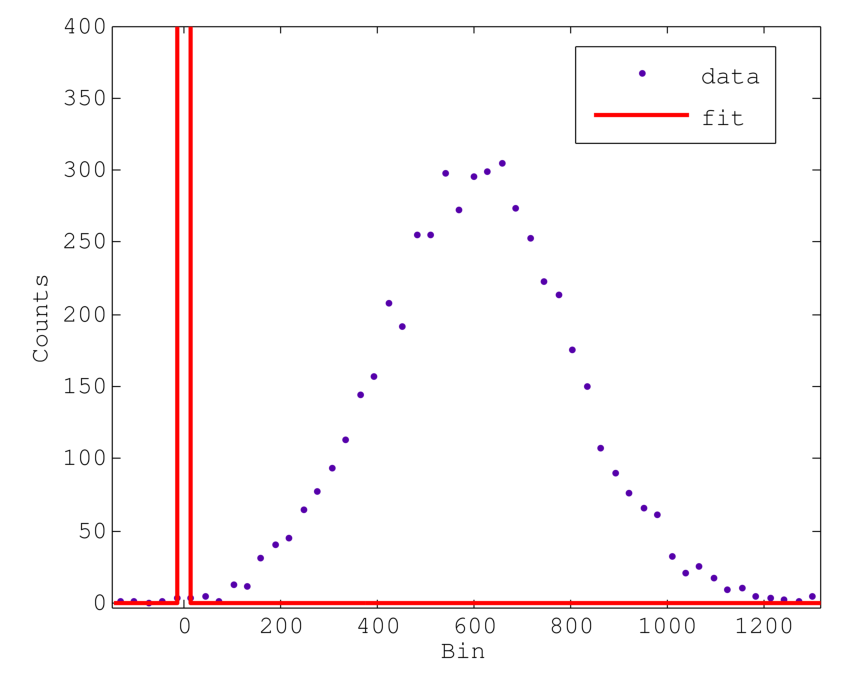
\includegraphics[scale=1]{gausnotwork.pdf}
 \caption{Fitting gaussian data generated on a computer with the function $ \mathtt{f(x)} =  \mathtt{a1}*\mathtt{exp}(-((\mathtt{x-b1})/\mathtt{c1})^\wedge \mathtt{ 2})$ in MATLAB. Choosing initial conditions of $\texttt{a1} = 1, \texttt{b1} = 0, \texttt{c1} = 1$, the computer algorithm that tries to minimize $\chi^2$ diverges.}
  \label{gausnotwork}
 \end{figure}
\end{center}
To fix this problem, and{ \it in general whenever you start any nonlinear fit}, it is a good idea to calculate a ballpark estimate of where the parameters should end up. In the example above, we know that the peak of the gaussian function should be about 300 high and located somewhere around 600 with a standard deviation on the order of 200. If we just start with parameters decently close to their final outcome, e.g. $\texttt{a1} = 300, \texttt{b1} = 600, \texttt{c1} = 200$, we get the following fit output:
\begin{framed}
\begin{verbatim}
General model Gauss1:
     f(x) =  a1*exp(-((x-b1)/c1)^2)
Coefficients (with 95% confidence bounds):
       a1 =   296.88732  (290.61741, 303.15724)
       b1 =   603.50693  (598.73503, 608.27883)
       c1 =   276.73864  (269.98996, 283.48732)

Goodness of fit:
  SSE: 3605
  R-square: 0.9934
  Adjusted R-square: 0.9931
  RMSE: 8.758
\end{verbatim}
\end{framed}
And the plot looks \emph{much} better:

\begin{center}
\Large \avantfont{ Good model with a good fit}

 \begin{figure}[H]
 
 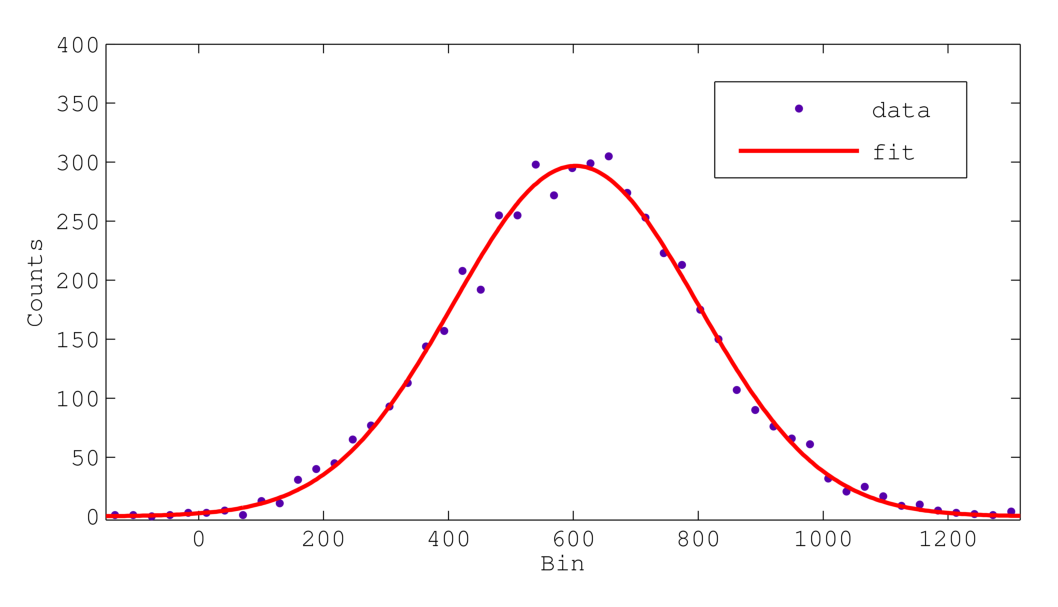
\includegraphics[scale=.9]{gauswork.pdf}
 \caption{Fitting gaussian data generated on a computer with the function $ \mathtt{f(x)} =  \mathtt{a1}*\mathtt{exp}(-((\mathtt{x-b1})/\mathtt{c1})^\wedge \mathtt{ 2})$ in MATLAB. Choosing initial conditions of $\texttt{a1} = 300, \texttt{b1} = 600, \texttt{c1} = 200$, the computer algorithm that tries to minimize $\chi^2$ settles to a good estimate.}
  \label{gauswork}
 \end{figure}
\end{center}
Now that we have a good fit, how can we use the fit output in a physics paper or report? The output that is produced is in the confidence interval format, which is a perfectly reasonable format to quote. For example, you could say:
\begin{framed}
``After fitting the data with a gaussian using a trust-region nonlinear least squares algorithm (default in MATLAB), we found the peak parameter $b$ converged to a value of 604 within a 95\% confidence interval (599, 608)."
\end{framed}
How do we decide what significant figures to use when the computer, when run long enough, could calculate 95\% confidence intervals out to 500 decimal places? It's not the lowest number of significant figures in the data, because the point of a fit is to reduce uncertainty by means of statistical analysis. The answer is that the confidence interval \texttt{(598.73503, 608.27883)}, as a measure of uncertainty, determines to what extent the parameter value \texttt{603.50693} is useful. The confidence interval can be expressed alternatively as \texttt{603.50693 (+ 5.7719, -  4.7719)}, at which point it becomes clear that everything after the ones' place is not useful (the uncertainty is of order 10$^0$. Now to get to an answer in the usual format of $\hat \mu \pm \hat \sigma$ must first convert to 68\% confidence (1$\sigma$) intervals by dividing the deviations by $1.96$. This is because a 95\% of a normal distribution lies between $-1.96\sigma$ and $+1.96\sigma$. So, enforcing significant figures, the value of \texttt{604 $\pm$ 5} at the 95\% confidence level becomes \texttt{604 $\pm$ 3}
at the standard 68\% confidence level.
\begin{framed}
{\bf In summary, if you are having problems with fitting, there are really only two things that can go wrong: either you're not looking for a minimized $\chi^2$ in the right place or you're using the wrong model.}
\end{framed}

\section{Evaluating Fits -- reduced $\chi^2$}
If you don't have the right model, how do you know in what way it's wrong? Well, there are really only two ways in which a model can be wrong.
\begin{enumerate}
\item {\bf The model oversimplifies the experiment.} When you haven't taken all of the physics into account, and your model at best only roughly approximates the data you've collected, there will likely be no combination of parameters that fit the data very well. 
\item {\bf The model overcomplicates the experiment.} When you have taken the physics of the experiment into account, and use extra parameters to describe the data, you will likely find a few combinations of parameters that work to describe the data very well. This means that the complexity of your model is {\it artificial} and does not reflect reality.
\end{enumerate}
To see whether the model is appropriate, physicists use a tool called reduced chi-squared ($\chi^2_{\text{red}}$). This is a quantity which represents the ratio of the estimated uncertainty in the model fit to the estimated uncertainty from experiment. Recall that $\chi^2$ was defined earlier as:
\begin{equation}
\chi^2= \sum_i \bigg (\frac{y_i - \hat y_i}{\hat \sigma_i} \bigg )^2
\end{equation}
Since $y_i - \hat y_i$ is the deviation of the data point $y_i$ from the model fit $\hat y_i$, and $\hat \sigma_i$ is the uncertainty calculated for the experiment at that data point, the contribution of any datapoint to $\chi^2$ is near one when the deviation of the model is about the same size as the uncertainty. What this means is that if we divide $\chi^2$ by the number of datapoints and get something close to one, then we can say that our model is good so long as we are confident in our estimate of uncertainty. Just like with Bessel's correction of the estimated standard deviation however (eq. \ref{bessel} ), we can't simply divide by the number of data points we have -- we have to divide by the \emph{degrees of freedom} $\nu = N - k - 1$.
\begin{equation}
\chi^2_{\text{red}} =   \frac{1}{\nu} \sum_i \bigg (\frac{y_i - \hat y_i}{\hat \sigma_i} \bigg )^2 = \frac{\chi^2 }{\nu}
\end{equation}
 As before, $N$ is the number of data points and $k$ is the number of parameters in the model. Of course, if $k+1 \ll N$, then this correction doesn't make much difference (it is however formally correct). When we accept $\chi^2_{\text{red}}$ as a good estimate of the ratio of model deviation to expected deviation, we can evaluate whether the model is good by examining the following cases:
 \begin{framed}
 \begin{easylist}[enumerate]
 & $\chi^2_\text{red} \gg 1$ . When the reduced chi-squared of a fit is much larger than one, the only possible ways for this to happen are for:
 && the model to fit so poorly that $(y_i - \hat y_i)^2 \gg (\hat \sigma_i)^2$ on average.
 && the uncertainty $ \hat \sigma_i$ to be so underestimated that $(y_i - \hat y_i)^2 \gg (\hat \sigma_i)^2$ on average, \emph{even though} the model fits fairly well. This is only practically possible if you think you have much more precision on your individual measurements than you \emph{actually} do. 
 & $\chi^2_\text{red} < 1$. When the reduced chi-squared of a model fit is less than one, the only way for this to happen is for the error in your fit to be overestimated so that $(y_i - \hat y_i)^2 < (\hat \sigma_i)^2$  on average. 
 \end{easylist}
 \end{framed}







% BAD STARTING POINTS
%General model Gauss1:
%     f(x) =  a1*exp(-((x-b1)/c1)^2)
%Coefficients (with 95% confidence bounds):
%       a1 =   100.00000
%       b1 =     1.00000
%       c1 =     0.00000
%
%Goodness of fit:
%  SSE: 1.048e+06
%  R-square: -0.913
%  Adjusted R-square: -0.9944
%  RMSE: 149.3
%
%  Warning: A negative R-square is possible if the model
%           does not contain a constant term and the fit
%           is poor (worse than just fitting the mean).
%           Try changing the model or using a different StartPoint.
% GOOD STARTING POINTS
%General model Gauss1:
%     f(x) =  a1*exp(-((x-b1)/c1)^2)
%Coefficients (with 95% confidence bounds):
%       a1 =   296.88721  (290.61729, 303.15712)
%       b1 =   603.50687  (598.73496, 608.27877)
%       c1 =   276.73886  (269.99018, 283.48755)
%
%Goodness of fit:
%  SSE: 3605
%  R-square: 0.9934
%  Adjusted R-square: 0.9931
%  RMSE: 8.758
%
%\subsection{Drosg's Seven Myths in Error Analysis}
%
%
%\begin{enumerate}
%\item Random errors can always be determined by repeating measurements under identical conditions.
%\item Systematic errors can be determined inductively
%\item Measuring is the cause of all errors
%\item Counting can be done without error
%\item Accuracy is more important than precision
%\item It is possible to determine the sign of an error
%\item It is all right to ``guess'' an error
%\end{enumerate}

%----------------------------------------------------------------------------------------
% Computational tools for physics
%----------------------------------------------------------------------------------------

\chapterimage{chapter_head_1.pdf} % Chapter heading image

\chapter{Mathematica, MATLAB, and Python}


\section{Computational tools in physics}

The next three chapters will be on the basic features of Mathematica, MATLAB and Python. These are three of the most common platforms broadly used for data analysis in physics. There certainly are other platforms that physicists use, but they are most often used in particular subfields (e.g. ROOT for high energy physics) even if they are broadly applicable. This chapter will serve as a guide to Mathematica, MATLAB, and Python because those platforms are available either in the PMCL and via student license (Mathematica and MATLAB) or can be downloaded for free (Python).



\begin{center}
{\renewcommand{\arraystretch}{1.2}
    \begin{tabular}{ |  p{1.5 cm}|| p{4 cm } | p{4 cm} || p{4 cm}|}
   \hline
	Feature &	\avantfont	{Mathematica} & \avantfont	{MATLAB} & \avantfont	{Python} \\ \hline \hline
	Syntax & Designed to be user-friendly and `like english', but non-conventional and maybe awkward at first & Inflexible but robust and easy to use & More complicated (it's actually a programming language) but relatively straightforward. \\ \hline
	Purpose & All-encompassing primarily symbolic platform for mathematical sciences & All-encompassing primarily numerical platform for experimental and engineering applications & A fast interpretted language with broad functionality and a relatively shallow learning curve. \\ \hline
	Coverage & Covers most analysis techniques but is somewhat weak and the error messages can be difficult to interpret. & Without the toolboxes, it is only useful if you download scripts or are willing to write them yourself. With the toolboxes (\$\$), it is excellent. & Covers everything that you would want to do with data analysis, but requires an understanding of the language to use. \\ \hline
	\end{tabular}		}
\end{center} 

\section{Learning these programs fast}

The eternal rule of learning to use any technology is
\begin{center}
\begin{framed}
\bf \Large{Learn to use the documentation}
\end{framed}
\end{center}
Learning how to use the documentation in the program or device you are using is essential to making progress with it. Reading about the platform is often the only alternative to guessing. Unfortunately

\begin{framed}
\texttt{Sample0001.txt} is a plain text file of numbers that can be downloaded from the SPS website. The first column is time
in some units. The rest of the columns have the x,y, and z components of the position of a few particles from a simulation. In this exercise you will preform various calculations, plots and analysis of this data. \\ 
\begin{enumerate}
\item Load the data from \texttt{Sample0001.txt} into a matrix
\item Plot a few of the columns of data as a function of column 1 (the time).
\item Compute the mean and standard deviation of all the columns after the
first.
\item Are the results for the x, y and z coordinates different? Are the results for
the different particles different? Answer this question quantitatively.
\item Make a histogram plot of columns 2 and 5. What is the connection between
these plots and question 2?
\item Make a parametric plot of columns 2 and 3 versus the time. The points in
your plot should be connected by lines.
\item Fit the plot from question (4) to a Gaussian function. Your can check your
fit parameters since they should have an obvious connection to the results from
(2). Is a Gaussian a good fitting function?
\item Your time series plots from question 1 have some clear oscillations. Take
the Fourier transform of this data and plot it.
\item Suggest what physical situation the data is computed for.
\item Do some other operation on the data of your choosing. For example, are
there any correlations between the position coordinates for particles 1 and 2?
\item Merit badge question: the parametric plot is messy because there are a
lot of data points. Plot the data such that the first batch of points is one color,
the next batch is another, etc. A half dozen colors should be enough: move across
the spectrum, red to blue, as you plot the data.
\end{enumerate}
\end{framed}
%----------------------------------------------------------------------------------------
%	Using Mathematica for Data Analysis
%----------------------------------------------------------------------------------------

\chapterimage{chapter_head_1.pdf} % Chapter heading image

\chapter{Using Mathematica for Data Analysis}

Besides being a great program for doing complicated algebraic calculations and working the calculus we're too lazy or pressed for time to slog through, Mathematica is a great program for basic plotting and fitting, and has many built in features which can instantly render figures and tables for use in a paper or lab report.


\section{Running commands}
\begin{remark}
If you've never used Mathematica ever before in your life, it may be useful to read this section.
\end{remark}
Mathematica is structured so as to act like a notebook you write down your equations in and manipulate your theoretical ideas. To make the feel of this program work, the software does not run like an ordinary scripting language. Instead of writing a program and executing a file, Mathematica evaluates one line at a time. This has some advantages, as you can change everything on the fly, but it may be confusing at first if you've never seen it before or are expecting to ``compile'' the whole program.

\subsection{Conventions}
 When entering commands in Mathematica, a few command conventions hold:
\begin{enumerate}
\item Commands always begin with capital letters and use square brackets (\texttt{[]}) are used for command arguments or as locations in a matrix when used twice ( e.g \texttt{[[]]})
\begin{example} Function arguments: \texttt{ListPlot[]}, \texttt{Table[]} \end{example}
\begin{example} Location in a matrix or ``table":  \texttt{A[[1,2]]} refers to the element in the first row and second column of matrix \texttt{A} \end{example}
\item Parentheses are used to group terms in an equation or an expression and are \emph{not} used in functions or denoting function arguments at all.
\item Greek letters like $\alpha$, $\beta$, $\gamma$ etc. are obtained by sandwiching the corresponding roman letters between escape characters. For instance, press escape then the letter \texttt{a} followed by escape again -- you should get $\alpha$. 
\end{enumerate}


\section{Loading data}
\begin{sloppypar}
Two common ways to import data are the \texttt{Import["file.txt","Format"]} and the \texttt{ReadList["file.txt","Format"]} functions.  On the computers in the PMCL, Mathematica will look specifically in your Documents folder for the data file you specify. One way to check whether this is true (it {\it might not be}) is to execute  the command \texttt{Directory[]}: this command will tell you where Mathematica is looking for files. However, if you give Mathematica the full file path, it will know exactly where to go.
\end{sloppypar}
Once your data files are in this folder (e.g. \texttt{"C:\textbackslash Users\textbackslash}$uteid$\texttt{\textbackslash Documents"}), you can simply use \texttt{Import[]} and \texttt{ReadList[]} without providing the full file address. This is a fast way to work if you like to download your files off of your email and continually send the updated versions to yourself. If you have a flashdrive however, a much more efficient solution can be found in useful tip \ref{UTuploadingdata}

\begin{example}
\texttt{rawdata = Import["Filewithdata.txt", "Table"];}
\end{example}
\begin{example}
\texttt{rawdata = ReadList["Filewithdata.txt", Number, RecordLists}$\to$\texttt{True];}
\end{example}

\begin{exercise}[Probably the most convenient solution to uploading data]


If you would like to change directories, for instance if you like to work off of a flash drive, you can quickly access files that are in the same folder as your notebook by using the \texttt{NotebookDirectory[]} command. The way to do this is by {\it concatenating} the notebook directory with the file name you're interested by using the \texttt{<>} between \texttt{NotebookDirectory[]} and \texttt{"Filewithdata.txt"}. The string you give Mathematica is then a complete filepath description of where the file is, and so this is very robust and useful. For example:

\begin{example}
If you have both your data file and your notebook file in a folder on a flash drive, let's call it \texttt{Flashdrive Folder}, and you want to import a text file with only comma-separated or tab-delimited data, you can use the following command and obtain a matrix with all of the data:\\\\
\texttt{rawdata = Import[NotebookDirectory[] <> "Sample0001.txt", "Table"];}\\ \\
Here, \texttt{NotebookDirectory[] <> "Sample0001.txt"} retrieves the string for the filepath \\ \texttt{I:\textbackslash Flashdrive Folder\textbackslash Sample0001.txt}. {\bf This means that every time you move \texttt{Flashdrive Folder}, Mathematica will be able to find the data files and you won't have any problems.}

If the file contains non-number (strings) in any of the columns, it is more useful to use the \texttt{Readlist[]} command as you can specify which columns don't contain numerical data. Let's say you have three columns in your \texttt{.txt} file where your first column specifies the date and the second and third  contain numerical data. By putting the list \texttt{\{Word, Number, Number\}} in as an option, Mathematica knows that the data in the first column are words and not numbers: \\
\\
\texttt{rawdata = }\\\texttt{  ReadList[NotebookDirectory[] <> "Sample0001.txt", \{Word, Number, Number\}]};\\
\\
In general, if you just want to input a datafile with only a matrix matrix, use:\\
\\
\texttt{rawdata =} \\ \texttt{ ReadList[NotebookDirectory[]<>"Sample0001.txt",  Number, }\texttt{RecordLists}$\to$\texttt{True];}
\end{example}
\label{UTuploadingdata}
\end{exercise}
%------------------------------------------------

\section{Plotting numerical data}\index{Figure}

To plot two columns of numerical data against eachother in Mathematica, you can't just give Mathematica two lists of data to plot. This is because the program likes to think of plotting numbers in terms of $\{x,y\}$ pairs. Instead, if you have a matrix ( \texttt{data}) with columns of numerical values imported correctly, you will have to construct a list of pairs. Once you get the hang of this, it can become reasonably intuitive. If you're used to Excel or MATLAB, it might be confusing at first though.

\begin{example}\index{Plotting in Mathematica}
To plot data in column 1  against data in column 2 of an imported dataset \texttt{data}, use: \texttt{ListPlot[data[[All,\{1,2\}]], AxesLabel }$\to$ \texttt{\{"Column 1", "Column 2"\},}\\ \texttt{
 ImageSize $\to$ Large]}\\

\end{example}
At the end of the command, \texttt{AxesLabel} and \texttt{ImageSize} are {\it options} that Mathematica has built-in settings for. If you are ever confused about what these options do, search the documentation for the function you're using and click on ``details'' on that page. This should tell you everything you need to know about what the function can do.  


\begin{figure}[h]
\centering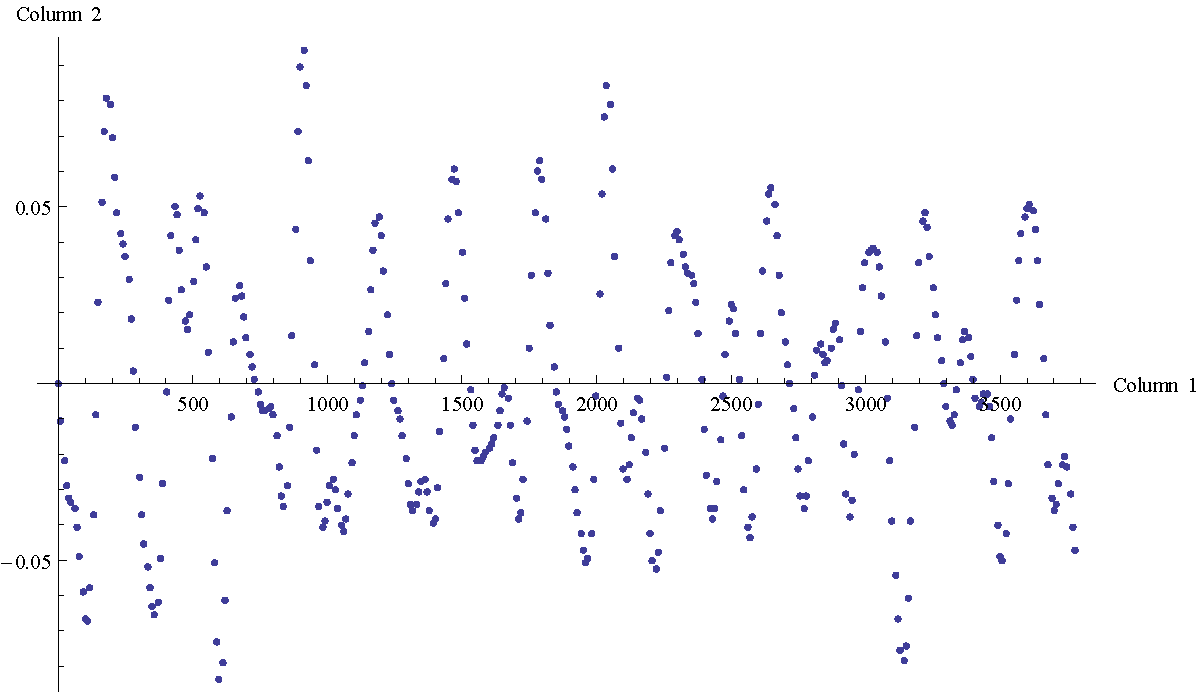
\includegraphics[scale=0.7]{listplot.pdf}
\caption{A \texttt{ListPlot[]} of sample data. One thing you may notice about this  plot is that it is rather cluttered and doesn't convey the fact that it is a timeseries very well. Also, the axes font isn't very readable at this scale.}
\end{figure}
To make the plot more readable, there are many options one can use in \texttt{ListPlot[]} or \texttt{ListLinePlot[]}. Some common options include:
\begin{enumerate}
\item {\bf Making axes font bigger:} \texttt{BaseStyle $\to$ \{FontSize $\to$ 20\}}, or whatever pt font you would like to use. The \texttt{BaseStyle} option includes ways of making the fonts bold or italic as well.
\item {\bf Titling plots:} \texttt{PlotLabel $\to$ "Title"} \texttt{PlotLabel $\to$ Style["Title", "Style"]}. Mathematica has a lot of style formats like `` Graphics'' and ``Section'' which mimic Mathematica's typsetting features. These can look pretty good at times, but it's a good habit to use \LaTeX $\;$ for plot titles if you can get that to work.
\item {\bf Adding grid lines:} \texttt{GridLines $\to$ Automatic}. This puts grid lines on the plot in a basic unassuming way. To make the lines dashed use \texttt{GridLineStyle $\to$ Dashed}. You can also specify where the grid lines are and change the color.

\end{enumerate}

\begin{figure}[h]
\centering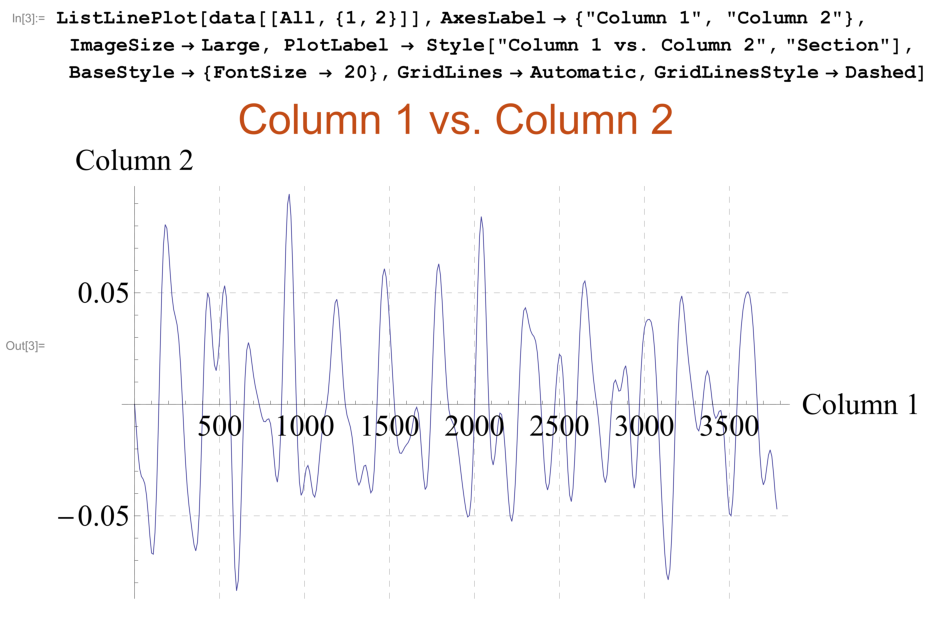
\includegraphics[scale=1]{complexplottingexample.pdf}
\caption{As you can see, this plot is more easy to look at and showcases the basic plotting options.}
\label{fig:listlineplot}
\end{figure}
\subsection{Histograms}
Making histograms is very straightforward using the \texttt{Histogram[$list$, $bins$]} command
\begin{figure}[H]
\centering 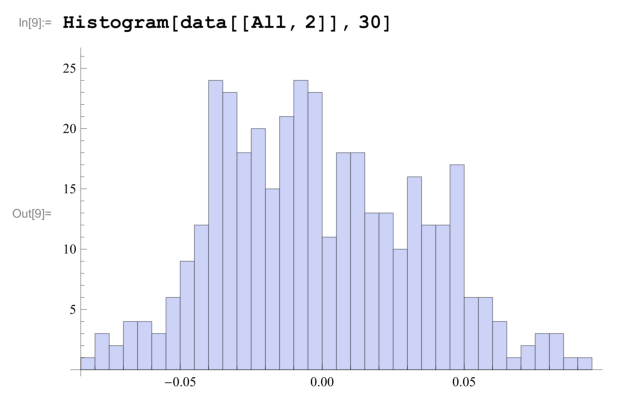
\includegraphics[scale=1]{histogramexample.pdf}
\caption{A histogram of a column of data}
\label{fig:histexample}
\end{figure}


\newpage
\section{Tables and Grids}
In mathematica, it is fairly straightforward to make a table of data with formatted headers. What mathematica needs to see is a matrix or list-of-lists of some form that can be put into a grid. In the example below, the code creates a column of means and a column of standard deviations for 18 columns of data, and then puts this information into a table with labelled columns and rows using the \texttt{TableForm[]} command:
\begin{figure}[H]
\centering 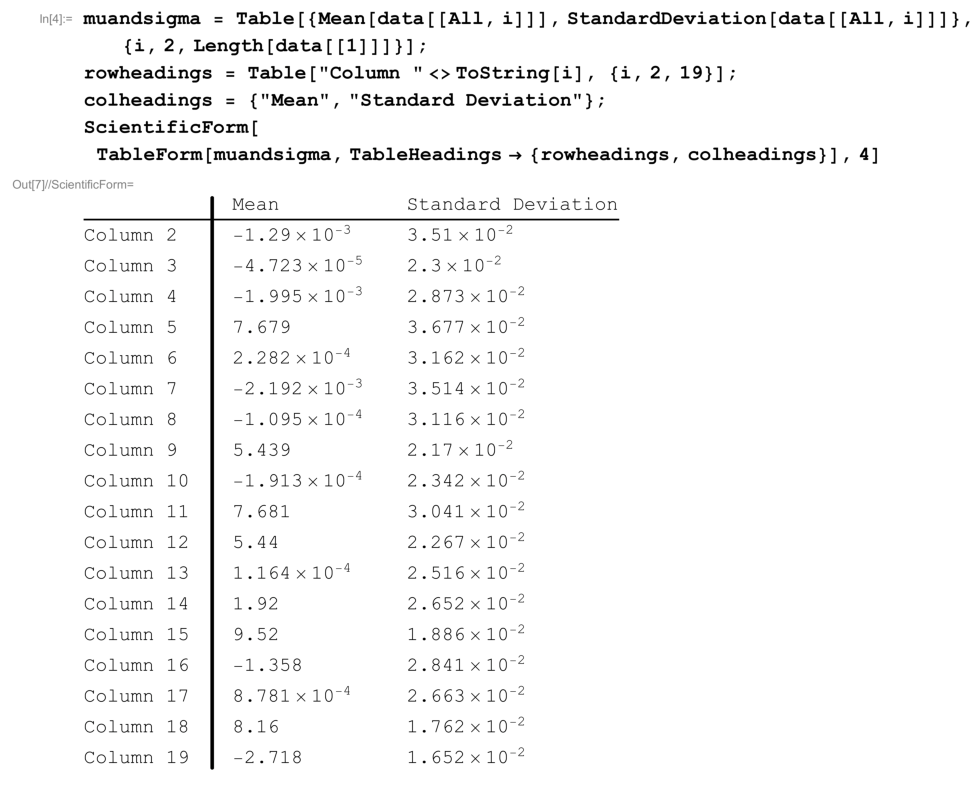
\includegraphics[scale=.97]{tableexample.pdf}
\end{figure}
\newpage
\section{Fitting arbitrary functions to data}
If you have some data and you are interested in fitting it with some nonlinear function, mathematica can do that without having to install a toolbox like MATLAB requires. The way to do this is to take some data and use the \texttt{NonlinearModelFit[]} command. In the example below, the data used in figure \ref{fig:histexample} is fit with a gaussian function. Because mathematica outputs a set of histogram bin edge positions instead of bin centers, the first four lines of the example are used to prepare a dataset that can be fit with a gaussian.
\begin{figure}[H]
\centering 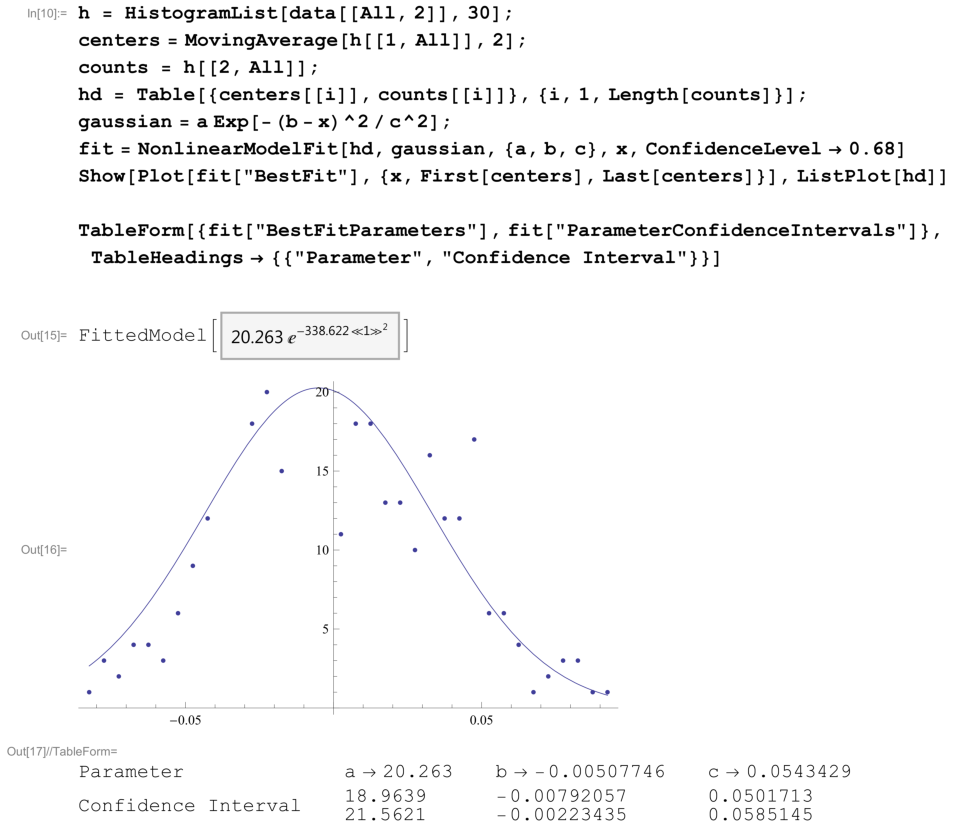
\includegraphics[scale=1]{basicfittingexample.pdf}
\end{figure}
This example again makes use of the \texttt{TableForm[]} command, useful for bundling the parameters and confidence interval informations into a table for easy reading. The general idea here is that \texttt{NonlinearModelFit[]} returns (creates) an object we decided to call \texttt{fit}.

\begin{exercise}[Interpretting this data: why \texttt{ConfidenceLevel} is important]
The parameters and confidence intervals of this model have been estimated using a nonlinear least-squares algorithm. This means that the uncertainties in the parameters have already been found, assuming that the noise in the data is uniformly distributed. So, if we want to read off uncertainties in the standard format of $\hat x \pm \hat \sigma_x$, all we need to do to find $\hat \sigma_x$ is divide the width of the confidence interval by two (the confidence interval takes up 2$\hat\sigma$). If \texttt{ConfidenceLevel$\to$ 0.95}, then the confidence interval would take up about 4$\hat \sigma$ instead. This comes from the standard normal distribution.
\end{exercise}
%----------------------------------------------------------------------------------------
%	Using MATLAB for Data Analysis
%----------------------------------------------------------------------------------------

\chapterimage{chapter_head_1.pdf} % Chapter heading image

\chapter{Using MATLAB for Data Analysis}
MATLAB stands for ``MATrix LABoratory'', which means that the program is on the one hand {\it extremely} good at working with matrices and on the other {\it somewhat limited} to those problems that can be solved using matrices. Naturally, if you spend some money and buy extra toolboxes it can do somewhat more elaborate calculations. In particular, the curve fitting toolbox is excellent and can do most if not all of the data analysis you might encounter in PHY 353L or PHY 474. In general though, if you are thinking about a problem and you can think of a way to quickly solve it using matrices and vectors, MATLAB is a good option. 

\begin{remark}
If you get MATLAB and think you might also buy the curve-fitting toolbox, you should get it at the same time as the main program since Mathworks updates their product very frequently (usually about twice per year), and if you have an academic license you can only get the most recent editions of the toolboxes online.
\end{remark}
\section{Introduction}
Since MATLAB is designed to work predominantly with lab data, it has many features which are tailored specifically to common tasks engineers and experimentalists do on a regular basis. For instance, the program has a file organizing system which can be viewed at any time and graphical user interfaces for common tasks like curve-fitting and importing data. Mathematica, on the other hand, is designed to encompass a much wider range of problems and so often falls short of MATLAB when it comes to convenience and ease of use in a laboratory setting.
\subsection{Scripts -- what makes MATLAB so popular}
When you want to do anything in MATLAB, you will always either use the buttons in the menus, or you will execute expressions through the `Command Window'. Because the expressions you might want to execute might be complicated and long, MATLAB has a file type (`.m') that it interprets as a long chain of commands. This is called a \emph{script} and is used widely in the MATLAB community to do a wide variety of computations.
When you open MATLAB you will see a few open `panes' in the program.
\begin{itemize}
\item{\bf Current Folder} -- This is where MATLAB looks for anything new (data, functions, scripts). If you're trying to load data make sure the `Current Folder' is looking at the file you're trying to use.
\item{\bf Editor} -- This is where you can edit and create new scripts and functions.
\item{\bf Workspace} -- This is the pane that displays all variables and their basic characteristics. This is very useful for checking up on variable characteristics.
\item{\bf Command Window} -- This is where expressions are executed. The most common things are functions, commands, and scripts.
\item{\bf Command History} -- This is where past expressions are stored so that you can access them easily. One very useful trick while coding in MATLAB is to press the `up' key on the keyboard to access the last command so you can edit it without having to write it out again.
\end{itemize}

The easiest ways to make a new script are (1) to press \texttt{Ctrl+N} while in the editor or (2) right-click on the Current Folder window and choose the `New File $\to$ Script' option. Once you have a \texttt{filename.m} file up, you can execute the entire file by simply typing \texttt{filename} in the command window.
\subsection{Syntax \& functions}

In MATLAB, commands \& functions are executed from the `command window'. Functions are of the form \texttt{functionName($arguments$)} in which case they call the \texttt{functionName} \emph{function}; commands are of the form \texttt{command $argument$}, in which case they run the \texttt{command} \emph{command}. In MATLAB, function inputs are always separated with commas and command inputs are always separated with spaces. Code is always interpreted in this way, which makes it easy to read. 
For instance:
\begin{example}[Command syntax]
\hfill \\
Some common examples of command syntax:
\begin{enumerate}
\item \texttt{clear all -except var1} clears all variables except for the variable named \texttt{var1}.
\item \texttt{load filename.mat} loads the variables saved to the {filename.mat} file.
\item \texttt{disp `This is a sentence which is also a string'} displays the sentence: \texttt{This is a sentence which is also a string}
\end{enumerate}
\end{example}

\begin{example}[Function syntax]
\hfill \\
Some common examples of function syntax:
\begin{enumerate}
\item \texttt{plot(x,y)} plots the vector \texttt{x} against the vector \texttt{y}, connecting each successive pair of points with a line segment \emph{note:} these vectors must be the same size.
\item \texttt{scatter(x,y)} plots the vector \texttt{x} against the vector \texttt{y} in a scatter plot, rather than connecting points.
\item \texttt{disp(a)} displays the object \texttt{a}, which might be a string, a matrix or some other object.
\end{enumerate}
\end{example}

To make a comment, just as in \LaTeX , you put a \texttt{\%} sign at some point in a line. Everything after that \texttt{\%} sign but before the next line gets commented out.
\begin{example}[Comments and displaying variables]
\hfill \\
Running the script:
\begin{framed}
\begin{verbatim}
% This is a comment and will not be displayed
a = [ 1 2 ; 4 5; 7 8]; % the matrix describing something important
b = [ 1 2 7 8]; % a vector  describing something important
disp 'The important matrix is:'; 	disp(a);
disp 'The important vector is:'; 	b
\end{verbatim}
\end{framed}
yields the output:
\begin{framed}
\begin{verbatim}
The important matrix is:
     1     2
     4     5
     7     8

The important vector is:

b =

     1     2     7     8
\end{verbatim}
\end{framed}
 In this way, you can get a script to output the answer to a calculation in a convenient format.
\end{example}


\subsection{Loading data}\label{loadingdata}
When you open the program, you will see a box on the left titled `Current Folder'. MATLAB can only see the files in your current folder, so this is where all your data files should go. Once a data file is in that folder, you can simply right-click the file and say `Import Data...'. Alternatively, you can go to the `File' menu and choose `Import Data...'. In either case you will end up in the same import wizard. You will be previewing the data to make sure it is in the right format. MATLAB is usually pretty good about identifying what kind of data you have (e.g. `comma-separated' or `tab-delimited'). 
Once you have your data imported into a matrix (the most convenient) or into a collection of differently named vectors, you can save the workspace into what is called a \texttt{.mat} file. This is MATLAB's special file format for saving workspaces. Now whenever MATLAB's current folder contains the your \texttt{data.mat} (assuming you named it \texttt{data.mat}), you can just use the \texttt{load data} command to import all the data that was in your workspace when you saved it.

\begin{exercise}[Importing multiple files ]
If you have a lot of files of the same type and you want them all to import the same way, one way to do that is to check the `Generate MATLAB Code' box in the import wizard. What this does is generate the code to import data of the form you specified in the prompt. If you save this code as `importfile' once it comes up, you will be able to use this command to import files quickly and reliably in a script.

This way you don't have to click through the wizard $n$ times if you have $n$ data files.%
\end{exercise}
\subsection{Plotting functions and data}
While in Mathematica, it is easy to tell the computer to plot a function against a dependent variable (or some other function of a dependent variable), MATLAB only understands vectors. This means that to plot $\sin(x)$ against $x$ for instance, you need to first decide which $x$ points you want. After you have an independent variable vector, and have the ability to construct a dependent variable vector (or if you already have two vectors of the same length), you can easily make a plot by calling the \verb|plot(xdata,ydata)| function.
\begin{framed}
\begin{verbatim}
x = 0:1e-2:2*pi;
plot(x,sin(x));
\end{verbatim}
\end{framed}
In the above code, the statement \verb| x = 0:1e-2:2*pi;| creates a vector of increasing values starting at \verb|0| and working up in increments of \verb|1e-2| ($1 \times 10^{-2}$) until the point \verb|2*pi|$=2\pi$ is reached. Again, once the domain of the function is created, it is easy to simply apply the sine function while creating the \texttt{plot()}. Note that a semicolon has been placed after each line -- the first is to keep the variable \verb|x| from being displayed, the second is for aesthetics. In general there's no harm in putting down a semicolon so use them everywhere.
\begin{figure}[H]
\centering
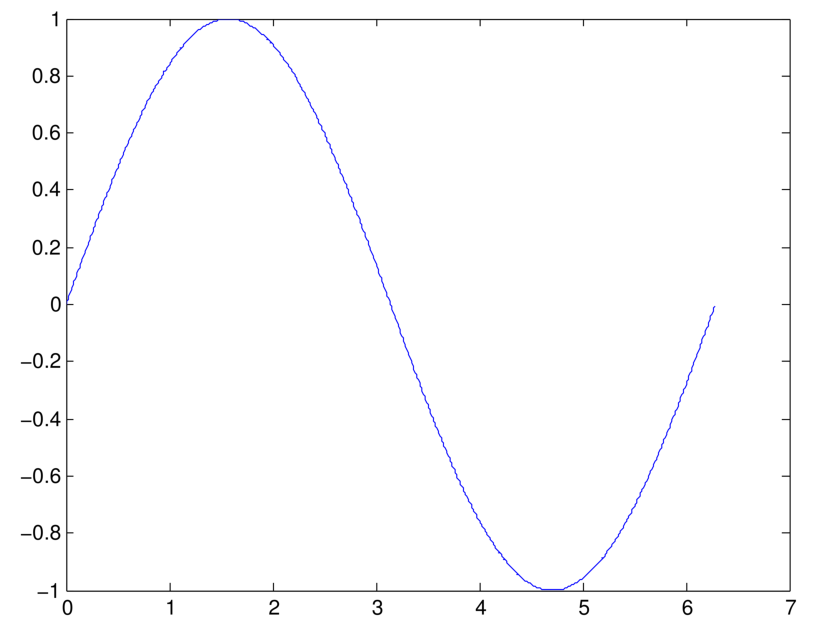
\includegraphics[scale=1]{sinplot.pdf}
\caption{Plot of \texttt{sin(x)} against \texttt{x}, where \texttt{x} is a $ 1 \times 629 $ vector from 0 to $2\pi$.}
\end{figure}
To plot data, it is often most convenient to have all your data in a matrix. It is a good practice to document your variables and how you name them somewhere. Documenting how the code you write is relevant to the experiment can easily be done with comments in the same file as your analysis using \texttt{\%} to create comments just as in \LaTeX. In the code below, the data has already been imported using the import data wizard mentioned 
in section \ref{loadingdata} and titled \texttt{data}. Fig. \ref{dataplot} shows the result:

\begin{framed}
\begin{verbatim}
plot(data(:,1),data(:,2));
xlabel('Column 1');
ylabel('Column 2');
title('Column 1 vs. Column 2');
\end{verbatim}
\end{framed}
\begin{figure}[h]
\centering
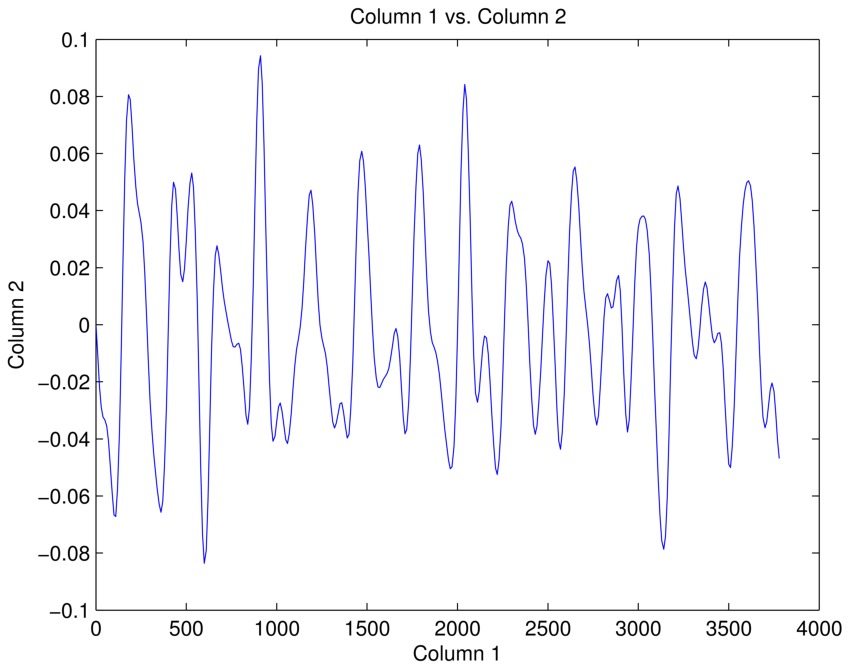
\includegraphics[scale=1]{p1e1.pdf}
\caption{Plot of one column of data (\texttt{data(:,1)}) against another (\texttt{data(:,2)}).}
\label{dataplot}
\end{figure}
This is the most basic kind of plot. However, often you may want to plot your data as points (in a scatter plot), rather than as a line plot. MATLAB has another function called \texttt{scatter()} which for two vectors works in exactly the same way as \texttt{plot()}. As in Mathematica, these functions are highly customizable.
\begin{remark}
In MATLAB there's a very nice way to customize plot which so long as you only have one plot is very easy and efficient. It is called the \emph{property editor}. You can get to it via the view menu if you have a plot open. It is a graphical user interface (GUI) with many options for titling plots, changing colors, sizes, line styles, etc.
\end{remark}

\subsection{Saving pictures}

If you're happy with your plot and want to put it into your paper you must first export it by going to \emph{Export Setup}. You can get to export setup through ``File $\to$ Export Setup" if you have an element on the figure selected in the Property Editor, or in the Property Editor window.\\

\emph{Remember:} you want to export files in the .pdf or .eps format as those do not have problems scaling when incorporated into a \LaTeX\ document.

\subsection{Histograms}

To make a histogram of a vector or matrix of data, the simplest thing is simply to write \texttt{hist(data)}. This will create a histogram plot with a number of bins that MATLAB thinks is appropriate. However, you can specify the number of bins with \texttt{hist(data,bins)} and if you would like to plot the bin centers against the bin counts, you can assign the output of the \texttt{hist} to two vectors representing this as in the example below:

\begin{framed}
\begin{verbatim}
[count, bin] = hist(data(:,2),30);
subplot(2,1,1); plot(bin,count);
title('Plot from Histogram Output');
subplot(2,1,2); hist(data(:,2),30);
title('Regular Histogram Plot');
\end{verbatim}
\end{framed}

\begin{figure}[h]
\centering
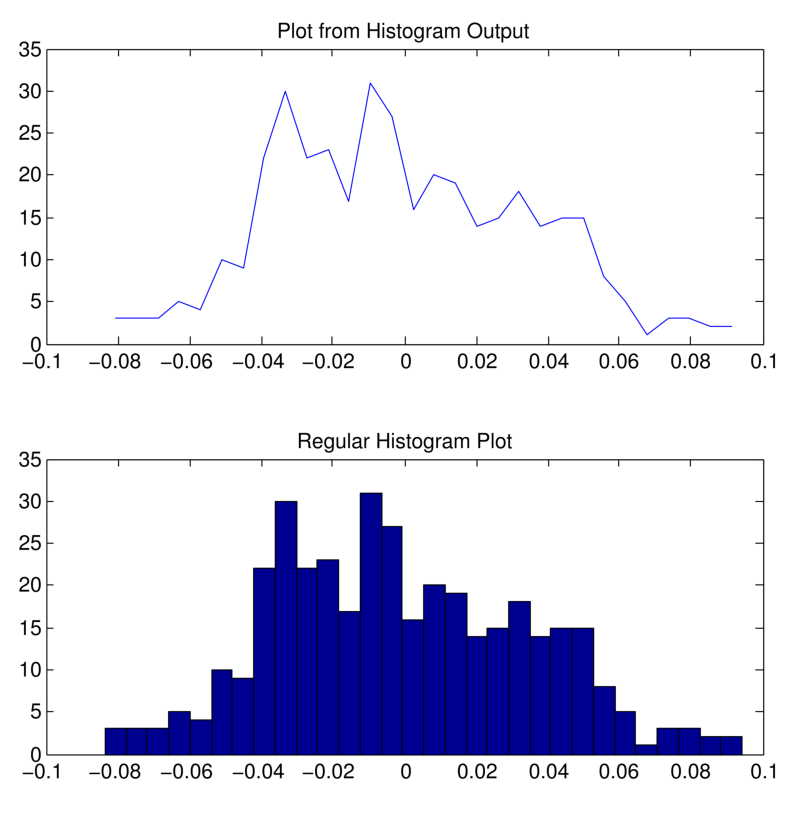
\includegraphics[scale=1]{histexample.pdf}
\caption{{Plots of the same histogram portrayed in two different ways. (Top) Histogram data is stored in two variables (\texttt{[count, bin]}) from the  \texttt{hist(data(:,2),30);} command which is a 30 bin histogram on \texttt{data(:,2)}. (Bottom) The traditional histogram from \texttt{hist(data(:,2),30);}. As you can see, \texttt{hist(data(:,2),30);} automatically outputs a plot unless you get output data from the function. If you were interested in how the data were distributed,\texttt{ [count, bin] = hist(data(:,2),30);} would be most useful because you could fit the \texttt{bin} and \texttt{count} with some distribution function (a gaussian for instance).}}
\label{histoplot}
\end{figure}


%%----------------------------------------------------------------------------------------
%	Scientific Writing
%----------------------------------------------------------------------------------------

\chapterimage{chapter_head_1.pdf} % Chapter heading image

\chapter{Scientific Writing}

\section{What constitutes a good scientific paper}






%----------------------------------------------------------------------------------------
%	BIBLIOGRAPHY
%----------------------------------------------------------------------------------------

\chapter*{Bibliography}
\addcontentsline{toc}{chapter}{\textcolor{ocre}{Bibliography}}
\section*{Books}
\addcontentsline{toc}{section}{Books}
\printbibliography[heading=bibempty,type=book]
\section*{Articles}
\addcontentsline{toc}{section}{Articles}
\printbibliography[heading=bibempty,type=article]

%----------------------------------------------------------------------------------------
%	INDEX
%----------------------------------------------------------------------------------------

\cleardoublepage
\setlength{\columnsep}{0.75cm}
\addcontentsline{toc}{chapter}{\textcolor{ocre}{Index}}
\printindex

%----------------------------------------------------------------------------------------

\end{document}